\documentclass[a4paper,fleqn]{cas-dc}

\usepackage[numbers,sort&compress]{natbib}
\usepackage{booktabs,multirow,tabularx}
\usepackage{amsmath,amssymb}
\usepackage{siunitx}
\usepackage{xcolor}
\usepackage{microtype}
\usepackage{enumitem}
\usepackage{graphicx}
\usepackage{algorithm}
\usepackage{algpseudocode}
\usepackage{placeins}

\newcommand{\method}{S-PA-CBB}
\newcommand{\rawmethod}{PA-CBB}
\newcommand{\logN}{\log_{10}N}
\newcommand{\dataset}[1]{\textsc{#1}}
\newcommand{\vect}[1]{\boldsymbol{#1}}

\begin{document}
\let\WriteBookmarks\relax
% Keep each result figure beside the question and interpretation that motivate it.
% Float-only pages are deliberately discouraged for the main manuscript.
\renewcommand{\topfraction}{0.95}
\renewcommand{\bottomfraction}{0.90}
\renewcommand{\textfraction}{0.05}
\renewcommand{\floatpagefraction}{0.95}
\renewcommand{\dbltopfraction}{0.95}
% Keep full-width figures on text pages; otherwise CAS may combine two figures
% on a dedicated float page even when dbltopnumber is one.
\renewcommand{\dblfloatpagefraction}{1.01}
\setcounter{topnumber}{2}
\setcounter{bottomnumber}{1}
\setcounter{totalnumber}{3}
% At most one full-width figure is admitted at the top of a physical page.
% Tables may share that page with the figure and the surrounding discussion.
\setcounter{dbltopnumber}{2}
\setcounter{dblbotnumber}{2}
\flushbottom

\shorttitle{From Physics to Selective Generation}
\shortauthors{Zhang et al.}

\title[mode=title]{From Physics to Selective Generation: Conditional Brownian Bridges for Sparse S--N Curve Reconstruction and Fatigue Decision-Making}

% --- Author information ---
\author[1]{Yunjian Zhang}[type=editor,orcid=0009-0002-8632-3996]
\ead{zhjunjian2024@lzu.edu.cn}
\credit{Conceptualization, Methodology}

\author[1]{Fuxiang Zhang}[type=editor,orcid=0009-0003-1462-2943]
\ead{zhangfx2023@lzu.edu.cn}
\credit{Conceptualization, Methodology, Data curation, Writing -- original draft}

\author[2]{Yixuan Li}[type=editor,orcid=0009-0002-6176-8331]
\ead{lyx2024@lzu.edu.cn}
\credit{Investigation, Validation}

\author[1]{Hubin Yang}[type=editor,orcid=0009-0004-0924-8974]
\cormark[1]
\ead{yanghb2019@lzu.edu.cn}
\credit{Supervision, Project administration, Funding acquisition}

% --- Affiliations and corresponding author ---
\affiliation[1]{organization={School of Information Science and Engineering, Lanzhou University},
  city={Lanzhou},
  postcode={730000},
  state={Gansu},
  country={China}}

\affiliation[2]{organization={School of Management, Lanzhou University},
  city={Lanzhou},
  postcode={730000},
  state={Gansu},
  country={China}}

\cortext[cor1]{Corresponding author: Hubin Yang (yanghb2019@lzu.edu.cn).}

\begin{abstract}
Dense S--N characterization consumes specimens and long-duration tests, yet early materials decisions are often made from only two to four failures. The sparse curves separate naturally into two regimes: a single-slope Basquin state is already informative for many cases, while knees, curvature and one-sided support create a difficult subset whose engineering quantities depend on the missing curve shape. We cast completion as a selective transformation problem and introduce a two-stage selective physics-anchored conditional Brownian bridge (\method). Stage~I scores curve difficulty from sparse support and a provisional bridge posterior. Stage~II retains the physical mean for physics-sufficient curves and applies a validation-shrunk residual transformation to the difficult subset, preserving posterior deviations and cross-stress covariance in both paths. Under identical sparse masks, \method{} achieves the lowest hidden-point error in all nine pooled database--budget settings across AM2022, CMA2022 and Weld2025. Target-excluded leave-one-database-out evaluation retains the advantage in eight of nine settings, with gains increasing as CMA2022 moves from two to three and four observations. Selective correction reduces raw-generator complete-grid error in every held-out database setting, while repeated samples improve proper distributional scores and stabilize covariance-guided experiment selection. Split-conformal calibration converts the generated spread into coverage-controlled intervals. The resulting framework links sparse physical fitting, selective residual generation and engineering decisions in one complete-curve representation.
\end{abstract}

% Highlights are submitted as a separate file in the Elsevier workflow. Keeping
% them out of the manuscript prevents the class from creating a sparse cover page.

\begin{keywords}
fatigue life \sep S--N curve \sep selective transformation \sep difficulty screening \sep Brownian bridge \sep active fatigue testing
\end{keywords}

\maketitle

\section{Introduction}

An S--N curve compresses a costly fatigue programme into a form that engineers can invert for fatigue strength, integrate for damage and interrogate when choosing the next specimen. The low-stress portion is especially expensive because failures may require millions of cycles. New alloy states, build orientations, heat treatments, surface conditions and load ratios multiply that burden. Basquin's log--log relation remains the natural first description of this curve \cite{Basquin1910}, while modern reviews place it within a broader family of stress--life and probabilistic design models \cite{Santecchia2018FatigueReview,Tridello2022PSNReview}. Bayesian and probabilistic formulations quantify slope and scatter from limited tests \cite{Li2020PSNInference,Barbosa2019ProbabilisticSN}. Sparse-data methods further improve parameter inference and design reliability \cite{Zhao2020SparseBayesianSN,Zhao2023BayesianSN}, and recent reviews summarize their role across fatigue regimes \cite{Kufoin2024ProbabilisticReview}.

Materials screening creates a sharper version of this problem. Two to four failures may be available, yet the required outputs---fatigue strength at a design life, remaining life at a service stress, integrated damage and the next informative stress---depend on the entire curve. Machine-learning reviews document the growing use of composition, process and loading descriptors in fatigue prediction \cite{Mirzaei2025MLReview,Reddy2025FatigueMLReview}. Representative models address general life regression and cracked components \cite{Prajapati2022AIFatigue,Wang2022CrackedML}, mean-stress and thermomechanical effects \cite{Zhu2022MeanStressML,Schafer2022TMFML}, and defect-aware or physics-constrained learning \cite{Salvati2022DefectPIML,Li2025HybridHCF}. Alloy-specific studies extend this progress to very-high-cycle fatigue and quantify predictive gains over physical baselines \cite{Shi2023VHCF,Wu2027PredictiveGain}. These approaches are effective point predictors; sparse curve completion adds the requirement that all stresses share one coherent conditional trajectory.

The key observation is that sparse completion has two physical regimes. Many curves remain close to a monotone single-slope relation, so the sparse Basquin fit already carries most of the useful structure. Curves with shoulders, knees, local curvature, regime-dependent slopes or one-sided observations contain a residual shape that moves engineering quantities. A flexible correction is valuable in this second regime and unnecessary in the first. Physics-informed learning provides the general principle of preserving known structure while estimating its discrepancy \cite{Karniadakis2021PhysicsML}. Physics-informed neural networks formalize this coupling between governing relations and learned fields \cite{Raissi2019PINN}, while materials machine learning shows the value of physically meaningful intermediate representations \cite{Butler2018MaterialsML}. We therefore organize sparse completion as a decision: assess the physical state, then transform the subset whose residual geometry carries additional information. Figure~\ref{fig:mechanism} summarizes this mechanism.

Conditional generation supplies the distribution required for that transformation. Denoising diffusion models learn complex conditional distributions through progressive corruption and reconstruction \cite{Ho2020DDPM}. Surveys describe their model families and practical design choices \cite{Yang2023DiffusionSurvey,Cao2024DiffusionSurvey}, while recent theory identifies the approximation errors that accumulate along the reverse trajectory \cite{Chang2024DiffusionTheory,Pierret2025DiffusionErrors}. Time-series diffusion extends these ideas to ordered one-dimensional signals \cite{Lin2024TimeSeriesDiffusion,Yang2026TimeSeriesSurvey}, and fast solvers reduce the number of network evaluations \cite{Lu2022DPMSolver}. Brownian-bridge diffusion is particularly suitable here because it connects two meaningful endpoints \cite{Li2023BBDM}; constrained inpainting shows how measured entries can remain fixed throughout sampling \cite{Lugmayr2022RePaint}. In our construction, the terminal endpoint is the sparse Basquin state, a one-dimensional U-Net resolves curve geometry \cite{Ronneberger2015UNet}, and a zero-initialized ControlNet path injects anchors and fatigue conditions \cite{Zhang2023ControlNet}.

The scientific value of generation lies in the distribution of complete trajectories. Proper scoring rules assess predictive distributions \cite{Gneiting2007Scoring}; interval scores measure calibration and sharpness \cite{Bracher2021IntervalScore}, and variogram scores probe dependence across stress locations \cite{Scheuerer2015VariogramScore}. Split-conformal prediction then maps validation residuals to coverage-controlled intervals \cite{Lei2018Conformal}. The resulting ensemble can support sequential experiments through its cross-stress covariance. Active-learning studies in materials already show how uncertainty can guide targeted measurement and discovery \cite{Lookman2019ActiveLearning,Balachandran2016ActiveMaterials}. Recent autonomous experimentation frameworks extend this principle to closed-loop materials campaigns \cite{Kusne2022ActiveLearning}, while critical evaluations emphasize matching the acquisition function to the scientific objective \cite{Liu2026ActiveLearningCritique}.

Three public resources provide distinct domains for testing this complete-curve view. AM2022 covers additively manufactured metals \cite{Zhang2023FatigueData}; CMA2022 contains metallic glasses and multi-principal-element alloys \cite{Zhang2023CMA}; Weld2025 contributes welded joints with geometry and treatment metadata \cite{Deng2025Welded}. We harmonize stress definitions and curve grouping, audit article- and curve-level duplicates, preserve database identity and evaluate both pooled and target-excluded transfer. This protocol connects the proposed mechanism to three questions: whether the selective correction improves hidden measurements, whether generated trajectories form a useful distribution, and whether that distribution changes an engineering decision.

\begin{figure}[pos=t]
\centering
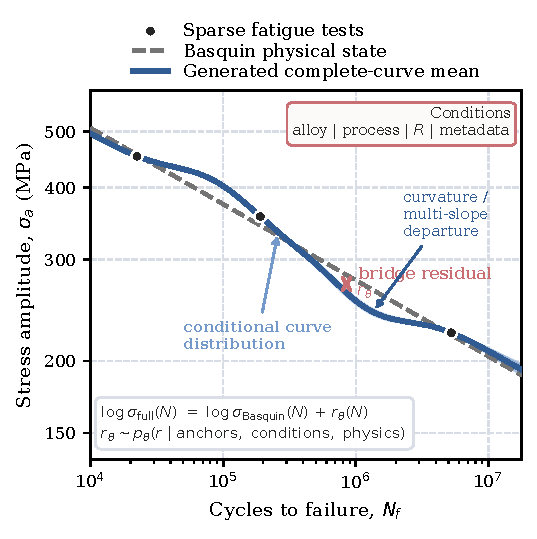
\includegraphics[width=\columnwidth]{figs/mechanism_explanation.pdf}
\caption{Conceptual mechanism of two-stage selective transformation. Sparse tests define a Basquin state and a difficulty assessment. Physics-consistent curves retain that state; flagged difficult curves receive a generated residual transformation and a distribution of complete S--N curves.}
\label{fig:mechanism}
\end{figure}

The study follows one central question: \emph{when should a sparse physical S--N state be retained, and when does a generated residual add engineering information?} Four contributions answer it:

\begin{itemize}[leftmargin=*,itemsep=3pt]
  \item A two-regime formulation separates physics-sufficient curves from curves requiring a structured residual transformation.
  \item A distributional audit combines proper scores, noise intervention, sample-count sensitivity, conformal calibration and cross-stress covariance.
  \item A mask-aligned three-database benchmark, true LODO evaluation and five downstream decisions connect reconstruction to fatigue engineering use.
  \item The resulting \method{} architecture joins a Basquin intermediate state, validation-fitted difficulty screening and a ControlNet-conditioned Brownian bridge that preserves posterior covariance along both decision paths.
\end{itemize}

Section~\ref{sec:method} specifies the model and inference algorithm. Section~\ref{sec:experiments} defines the data protocol, compact reconstruction benchmark and component check. Section~\ref{sec:downstream} reports the validation-selected engineering tasks and active experiment selection.

\section{Method}\label{sec:method}

\subsection{Problem definition and notation}

For fatigue curve $c$, let $s$ denote a scalar stress coordinate after conversion to a common MPa convention, $x=\log_{10}s$, and $y=\log_{10}N$ the log cycles to failure. The complete curve is represented on a monotonically increasing grid $\vect{x}_c=(x_{c1},\ldots,x_{cG})$ with $G=32$. Grid limits are curve-specific during preprocessing and are mapped to $[-1,1]$ for the network. The target vector is $\vect{y}_{0,c}\in\mathbb{R}^{G}$.

At test time, only $k\in\{2,3,4\}$ experimental failures are revealed. Their values are projected to the common grid, producing a sparse signal $\vect{o}_c$, a mask $\vect{m}_c\in\{0,1\}^{G}$ and the original off-grid coordinates used for exact evaluation. Curve-level metadata are encoded as $\vect{q}_c$. Depending on the database, $\vect{q}_c$ can contain alloy family, nominal composition, manufacturing route, heat treatment, surface treatment, load ratio, frequency, temperature, specimen class, weld category and stress-definition flags. Missing categorical values receive an explicit unknown token; continuous variables are accompanied by missingness indicators.

The desired output is the conditional distribution
\begin{equation}
 p_\theta(\vect{y}_0\mid \vect{o},\vect{m},\vect{x},\vect{q},\vect{y}_{\mathrm{phys}}),
 \label{eq:conditional}
\end{equation}
whose draws pass through the revealed observations after projection, remain compatible with the material/test condition and represent plausible full-curve shapes. The predictive mean, quantiles, fatigue strengths and acquisition scores are derived from the same ensemble.

\subsection{Overview and large workflow figure}

Figure~\ref{fig:workflow} is reserved for the final method diagram. The intended left-to-right flow is: three reported public databases; unit and definition harmonization; DOI/title/curve duplicate audit; source-disjoint split construction; sparse-mask simulation; Basquin physical-state estimation; ControlNet-conditioned Brownian bridge; ensemble of full S--N curves; conformal calibration; point, curve, distributional and downstream evaluation. The final artwork should visually separate information available during training from information available for a new sparse curve.

\begin{figure*}[t]
\centering
\fbox{\begin{minipage}[c][0.20\textheight][c]{0.95\textwidth}
\centering
\Large Workflow figure placeholder\\[12pt]
\normalsize Three databases $\rightarrow$ harmonization and duplicate audit $\rightarrow$ strict splits\\[6pt]
$\rightarrow$ sparse anchors and metadata $\rightarrow$ Basquin physical state\\[6pt]
$\rightarrow$ controlled Brownian bridge $\rightarrow$ complete-curve ensemble\\[6pt]
$\rightarrow$ conformal calibration $\rightarrow$ benchmark and downstream decisions
\end{minipage}}
\caption{Placeholder for the full method workflow. The final vector figure will distinguish offline database preparation, model training and inference for a new sparse curve. It will also show that external databases remain unavailable to the model in zero-shot evaluation.}
\label{fig:workflow}
\end{figure*}

\subsection{Data harmonization and curve construction}

The bridge requires comparable one-dimensional curves, so raw records pass through a definition-aware conversion layer. Stress amplitude is retained directly. Stress range is divided by two when the database explicitly reports a range and the load convention permits the conversion. Maximum stress is converted using the reported load ratio $R=\sigma_{\min}/\sigma_{\max}$, giving $\sigma_a=(1-R)\sigma_{\max}/2$. Ambiguous stress definitions are assigned to a separate stress-type domain or omitted from the common-amplitude benchmark. Reversals are converted to cycles when the original definition is explicit.

The completion likelihood uses failure points, while runouts remain marked as censored observations for consistency checks and future likelihood extensions. Within one database, points form a curve when material state, processing, specimen, environment, stress ratio, frequency and temperature agree at the available resolution. Curves require at least six failures, four unique stresses, log-stress span of at least 0.04 and a fitted negative slope in $[-25,-0.05]$. Replicates at the same stress are preserved for raw-data auditing; a robust centre constructs the 32-point reference representation.

Cross-database duplicates are detected hierarchically. Exact DOI matches are checked first, followed by normalized title and author/year matches. Candidate curves within matched articles are then compared by alloy, $R$, temperature, process labels and rounded $(S,N)$ pairs. Any matched record is assigned to one source group before splitting and is never counted as an independent test curve in another database.

\subsection{Basquin physical state}

The physical state is fitted exclusively from the revealed anchors. The Basquin relation can be written
\begin{equation}
 y=a+bx,\qquad b<0.
 \label{eq:basquin_v2}
\end{equation}
For $k\geq3$, $(a,b)$ are estimated by robust regression. For $k=2$, the two points identify a line but the slope can be unstable when their stresses are close. We therefore shrink the sparse slope toward a training-only conditional prior:
\begin{equation}
 \hat b=\lambda_c b_{\mathrm{sparse}}+(1-\lambda_c)b_{\mathrm{prior}}(\vect{q}),
 \quad
 \lambda_c=\frac{\Delta x_c^2}{\Delta x_c^2+\tau_b^2},
 \label{eq:slope_shrink}
\end{equation}
where $\Delta x_c$ is the observed log-stress span and $\tau_b$ is selected on the validation set. The intercept is then chosen to minimize robust anchor residuals. Slope clipping enforces negative, numerically stable extrapolation. Evaluation on the grid produces $\vect{y}_{\mathrm{phys}}$, the physical intermediate representation evaluated through component ablation.

The physical state serves three roles. First, it supplies a monotone low-frequency trend. Second, it provides an endpoint for the Brownian bridge, making the stochastic path conditional by construction. Third, it converts a hard absolute-learning problem into residual transport. The model must learn $\vect{y}_0-\vect{y}_{\mathrm{phys}}$, which is smaller and more comparable across strength scales than $\vect{y}_0$ itself.

\subsection{Brownian-bridge forward process}

Let $t\in(0,1)$ and $m_t=t$. A forward bridge between the complete curve and the physical endpoint is
\begin{equation}
 \vect{y}_t=(1-m_t)\vect{y}_0+m_t\vect{y}_{\mathrm{phys}}
 +\sigma\sqrt{m_t(1-m_t)}\vect{\epsilon},
 \quad \vect{\epsilon}\sim\mathcal{N}(\vect{0},\vect{I}).
 \label{eq:bridge_v2}
\end{equation}
The variance is zero at both endpoints and largest near the middle of the path. This differs from a conventional unconditional diffusion model, where the terminal state is approximately Gaussian noise. Here the terminal state is a physically interpretable curve, and reverse sampling transports that curve toward the conditional data distribution.

The network returns three length-$G$ heads: predicted noise $\hat{\vect{\epsilon}}$, a direct clean-curve estimate $\hat{\vect{y}}_0^{\mathrm{dir}}$, and log variance $\hat{\vect{v}}$. A score-derived clean estimate follows from rearranging Eq.~\eqref{eq:bridge_v2}. The direct and score-derived estimates are blended as a function of time: the direct head stabilizes early reverse steps near the physical endpoint, while the score-derived estimate receives more weight near the data endpoint.

\subsection{One-dimensional U-Net and control pathway}

The base network is a one-dimensional U-Net with base width 48 and three spatial resolutions. Each resolution contains residual convolutional blocks, group normalization and a time embedding. Downsampling expands the receptive field so that local anchor information can affect distant stresses; skip connections preserve location-specific detail. The final heads operate at the original 32-point resolution.

The control encoder mirrors the backbone encoder. Its channels concatenate the sparse grid values, observation mask, normalized coordinate, physical state and broadcast metadata embedding. Following the ControlNet principle \cite{Zhang2023ControlNet}, control residuals enter the frozen/pretrained backbone through initially zero-valued projections. The conditional branch therefore begins as an identity perturbation of the base transport process. In the second training stage, the control parameters and selected backbone layers are optimized jointly.

Metadata are encoded by type. Categorical fields use learned embeddings with an unknown category. Continuous fields are standardized using training statistics and paired with presence bits. Alloy composition, where available, is mapped to a fixed element vector; otherwise an alloy-family embedding is used. The principal zero-shot setting uses transferable material and test descriptors, while database identity is reserved for diagnostic domain-conditioning experiments.

At every reverse step, revealed observations are projected back into the current state. For an on-grid anchor, the replacement is exact. For an off-grid anchor, the two adjacent grid values are corrected by the minimum-norm linear update that makes their interpolation equal to the observation. This projection enforces observation fidelity as an algorithmic constraint.

\subsection{Training objective}

The loss combines four terms:
\begin{align}
 \mathcal{L}={}&\mathcal{L}_{\epsilon}
 +\lambda_0\mathcal{L}_{0}
 +\lambda_{\Delta}\mathcal{L}_{\Delta}
 +\lambda_{c}\mathcal{L}_{\mathrm{cons}},\\
 \mathcal{L}_{\epsilon}={}&\frac{1}{G}\sum_j
 \left[\exp(-\hat v_j)(\epsilon_j-\hat\epsilon_j)^2+\hat v_j\right],\\
 \mathcal{L}_{0}={}&\|\hat{\vect{y}}_0^{\mathrm{dir}}-\vect{y}_0\|_2^2,\\
 \mathcal{L}_{\Delta}={}&\|\Delta\hat{\vect{y}}_0^{\mathrm{dir}}-\Delta\vect{y}_0\|_1,\\
 \mathcal{L}_{\mathrm{cons}}={}&\operatorname{SmoothL1}
 (\hat{\vect{y}}_0^{\mathrm{dir}},\hat{\vect{y}}_0^{\mathrm{score}}).
 \label{eq:loss}
\end{align}
The heteroscedastic noise term learns location-dependent stochastic scale. The clean loss stabilizes the small-grid problem, and the first-difference loss discourages spurious oscillations while retaining multi-slope and plateau behaviour. A hard monotone projection is evaluated separately as a decision-time variant.

Training uses two stages. The base bridge is trained for 60 epochs. The control branch is then attached and trained for 80 epochs. AdamW uses learning rate $2\times10^{-3}$, weight decay $10^{-4}$, batch size 48 and gradient-norm clipping at 2.0. Sixteen sparse masks are sampled per training curve across $k=2,3,4$. Seeds fix the dataset split, mask stream and parameter initialization. Distributed training uses seven Ascend devices; synchronized per-curve inference latency is reported separately in the sampler ablation.

\subsection{Reverse sampling and posterior ensemble}

All main, external, leave-database-out and downstream results use one frozen sampler: three reverse steps, 32 independent trajectories and transition-noise scale $\eta=0.5$. The sampler begins exactly at the physical endpoint, whose Brownian-bridge variance is zero, predicts the clean state at each step, advances toward $t=0$, injects Gaussian stochasticity at non-terminal intermediate states and re-imposes the observed anchors. Split-conformal calibration is fitted on validation curves after fixing this sampler. Longer-step and ensemble-size sweeps serve as sensitivity analyses around the common headline protocol. Algorithm~\ref{alg:inference} specifies inference for one sparse curve.

\begin{algorithm*}[t]
\caption{Physics-anchored conditional generation for one sparse S--N curve}
\label{alg:inference}
\begin{algorithmic}[1]
\Require Observations $\mathcal{O}=\{(s_i,N_i)\}_{i=1}^{k}$; metadata $\vect{q}$; trained model $f_\theta$; grid size $G$; reverse steps $T$; ensemble size $M$
\Ensure Posterior samples $\{\vect{y}_0^{(r)}\}_{r=1}^{M}$ and calibrated intervals
\State Convert explicit stress/life definitions to $x_i=\log_{10}s_i$ and $y_i=\log_{10}N_i$
\State Construct grid $\vect{x}$, sparse signal $\vect{o}$ and observation mask $\vect{m}$
\State Estimate $(\hat a,\hat b)$ with Eq.~\eqref{eq:slope_shrink} and evaluate $\vect{y}_{\mathrm{phys}}=\hat a+\hat b\vect{x}$
\State Encode control tensor $\vect{h}=\operatorname{Encode}(\vect{o},\vect{m},\vect{x},\vect{q},\vect{y}_{\mathrm{phys}})$
\For{$r=1$ to $M$}
  \State Initialize $\vect{z}_{T}\leftarrow\vect{y}_{\mathrm{phys}}$ exactly at the physical endpoint
  \For{$j=T,T-1,\ldots,1$}
    \State $(\hat{\vect{\epsilon}},\hat{\vect{y}}_0^{\mathrm{dir}},\hat{\vect{v}})\leftarrow f_\theta(\vect{z}_j,\vect{h},t_j)$
    \State Compute score-derived $\hat{\vect{y}}_0^{\mathrm{score}}$ and blend the two clean estimates
    \State Advance $\vect{z}_{j-1}$ with the Brownian-bridge reverse update and predicted variance
    \State Project the revealed observations back onto $\vect{z}_{j-1}$
  \EndFor
  \State Store $\vect{y}_0^{(r)}\leftarrow\vect{z}_{0}$
\EndFor
\State Compute ensemble mean, raw quantiles and curve-derived downstream quantities
\State Apply validation-fitted conformal residual quantiles while preserving the generated mean
\State \Return posterior ensemble and calibrated prediction bands
\end{algorithmic}
\end{algorithm*}

\subsection{Stage I difficulty screening and Stage II residual transformation}

Unconditional residual generation can over-correct a curve whose sparse physical state is already adequate. The deployed model therefore treats completion as a two-stage decision. In Stage I, a provisional physics-anchored bridge posterior assesses difficulty. Prospective quantities available at inference---generated tail-residual magnitude, observed stress-span coverage and posterior spread---form a scalar score. A validation-fitted threshold $\tau_k$ maps that score to $g\in\{0,1\}$: $g=0$ denotes a physics-sufficient curve and $g=1$ denotes a curve requiring transformation. Gate fitting uses validation curves and prospective quantities exclusively.

Stage II either retains or transforms the physical state. Let $\{\vect{y}^{(r)}_{\mathrm{raw}}\}_{r=1}^{M}$ be the provisional ensemble, $\bar{\vect{r}}=M^{-1}\sum_r\vect{y}^{(r)}_{\mathrm{raw}}-\vect{y}_{\mathrm{phys}}$ its mean residual, and $\vect{d}^{(r)}=\vect{y}^{(r)}_{\mathrm{raw}}-\bar{\vect{y}}_{\mathrm{raw}}$ its zero-mean posterior deviations. For each sparse budget, the transformation strength $\alpha_k$ is also fitted on validation curves. The final posterior is
\begin{equation}
 \vect{y}^{(r)}_{\mathrm{sel}}=
 \vect{y}_{\mathrm{phys}}+g\alpha_k\bar{\vect{r}}+\vect{d}^{(r)}.
 \label{eq:selective_gate}
\end{equation}
Thus Stage I decides whether transformation is warranted, while Stage II applies a validation-chosen fraction of the residual and preserves stochastic deviations and cross-stress covariance. When $g=0$, the mean reverts to the physical state while uncertainty remains available for calibration and acquisition. When $g=1$, the difficult curve receives a structured residual transformation. The unconditional \rawmethod{} is retained as the ablation obtained by transforming every curve.

\subsection{Split-conformal calibration}

Raw ensemble quantiles are diagnosed before correction. For each target coverage $1-\alpha$, the validation set supplies nonconformity scores based on the distance of a held-out observation from the raw central interval. The finite-sample conformal quantile expands the lower and upper bounds symmetrically in $\logN$ space. Calibration parameters are fitted separately by sparsity level, and subgroup calibration is reported when its validation sample supports estimation. Expansion widths are fixed from validation data before test evaluation.

This separation assigns distinct roles to generation and calibration. The stochastic head supplies structured spread, while the conformal layer aligns empirical coverage with the requested level. Raw coverage, conformal coverage, interval width and interval score are reported together to quantify both calibration and sharpness.

\section{Experimental design and results}\label{sec:experiments}

\subsection{Three-database benchmark}

Table~\ref{tab:datasets} defines the role of every database. A common conversion and filtering pipeline maps the different release-level objects to eligible curve counts after local download and audit.

\begin{table*}[b]
\caption{Public fatigue resources after common curve construction. Release statistics are abbreviated; eligible curves are computed by the present preprocessing pipeline.}
\label{tab:datasets}
\centering
\scriptsize
\setlength{\tabcolsep}{5pt}
\renewcommand{\arraystretch}{1.05}
\begin{tabularx}{\textwidth}{p{3.0cm}X p{1.6cm} p{5.0cm}}
\toprule
Database & Scope & Eligible & Use \\
\midrule
FatigueData-AM2022 \cite{Zhang2023FatigueData} & Additively manufactured metals with process and test metadata & 1,015 & Development split and alloy-held-out tests \\
FatigueData-CMA2022 \cite{Zhang2023CMA} & Metallic glasses and multi-principal-element alloys & 105 & Cross-material and pooled evaluation \\
Welded-joint database \cite{Deng2025Welded} & Weld, geometry and post-treatment conditions & 2,817 & Large domain-shift evaluation \\
\bottomrule
\end{tabularx}
\end{table*}

For AM2022, the present filter retains curves with at least six non-runout failures, at least four distinct stresses, sufficient log-stress span and a negative fitted slope. Grouping by source paper yields 609 training, 203 validation and 203 test curves. No paper contributes to more than one split. The same test curve receives a fixed mask for every method, and metrics are computed on exactly the same hidden points.

External evaluation has two levels. The pooled benchmark estimates database-resolved performance under one harmonized training protocol. In \emph{leave-database-out} (LODO) evaluation, the target database is excluded from both training and validation; the held-out database is opened only after model, gate and correction-strength selection. LODO is reported for AM2022, CMA2022 and Weld2025 because each supports a database-level estimate.

\subsection{Data coverage and uncertainty structure}

The harmonized resources occupy different stress--life regions, while AM2022 and Weld2025 dominate the eligible-curve count. This imbalance makes macro-averaged, database-resolved reporting necessary: a pooled point average would otherwise be governed by the welded-joint resource.

Figure~\ref{fig:data_v2} summarizes the public-data condition space before model comparison. The parallel coordinates show curve support and test conditions, while the lower panels expose alloy, process and publication-year imbalance. These descriptors motivate source-aware splitting and prevent a large database from being mistaken for broad physical coverage.

\begin{figure*}[!t]
\centering
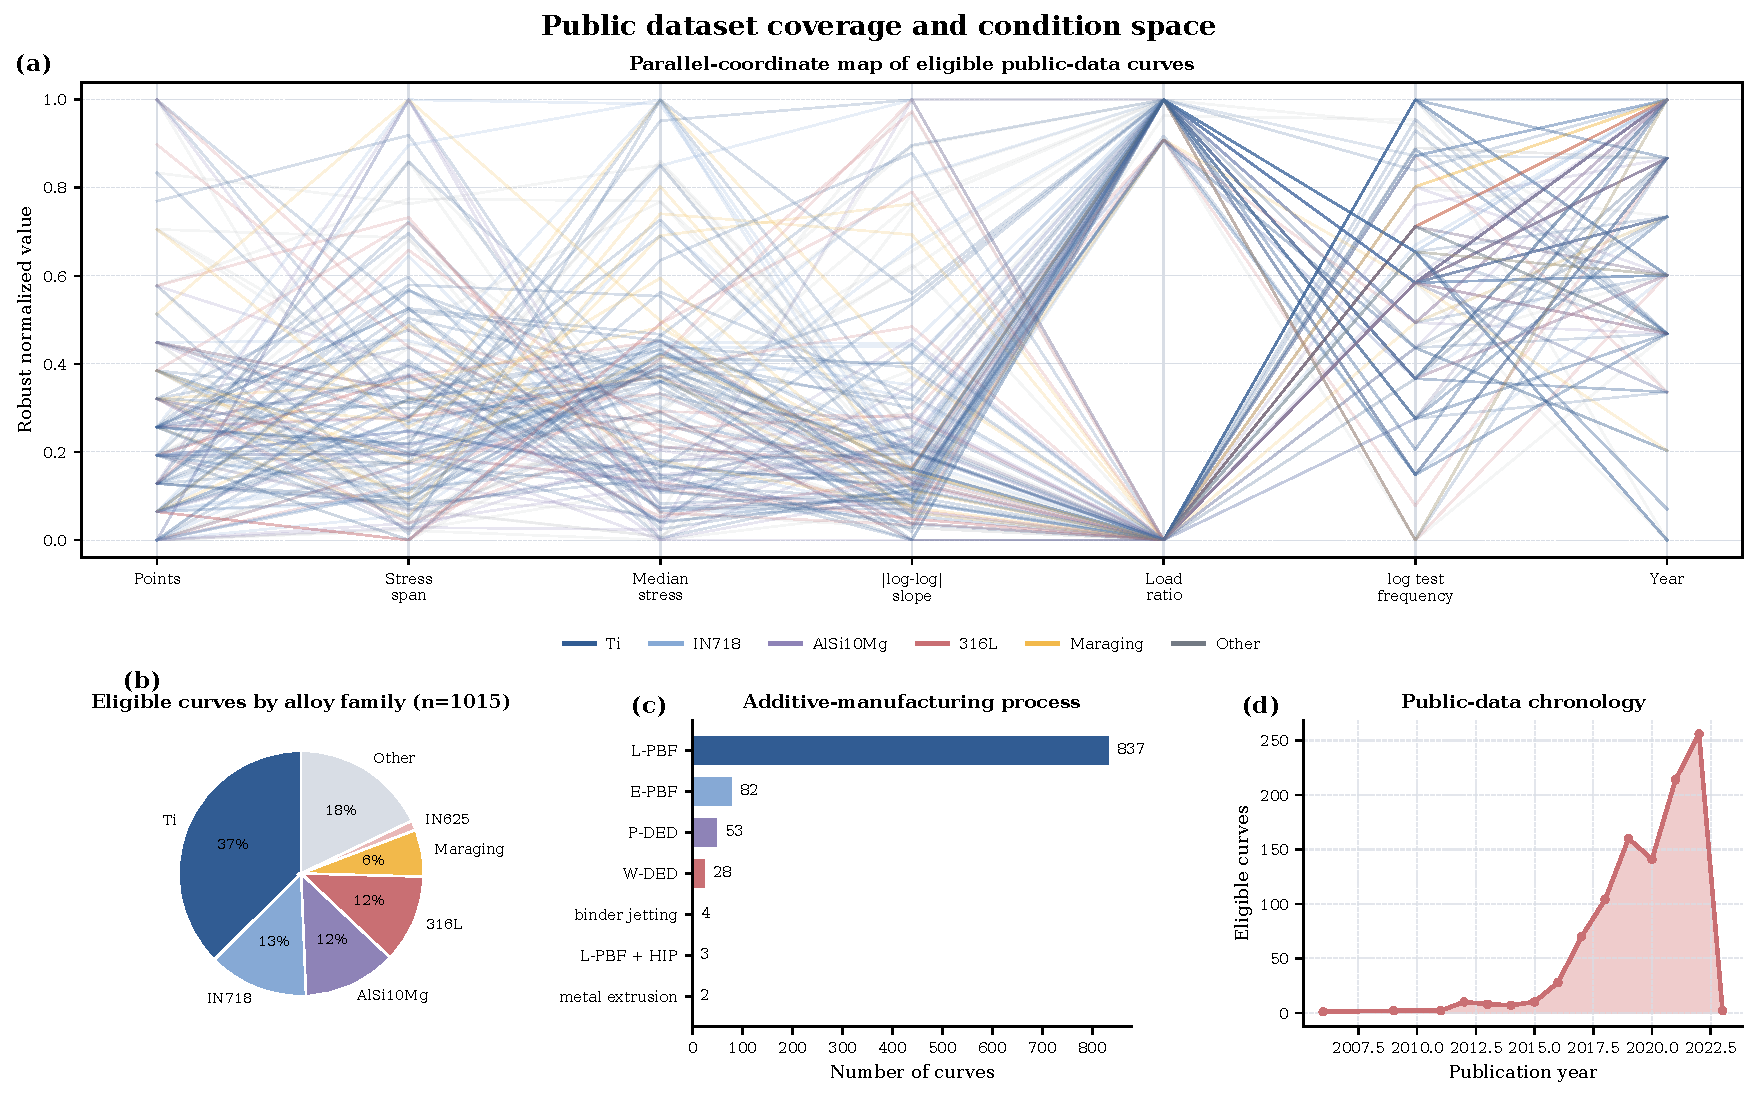
\includegraphics[width=\textwidth,height=0.38\textheight,keepaspectratio]{figs/dataset_map.pdf}
\caption{\textbf{Question: What condition space is represented by the public fatigue data?} The parallel-coordinate map summarizes curve and test descriptors; the lower panels show alloy-family composition, manufacturing routes and publication chronology. \textbf{Finding:} coverage is broad but strongly imbalanced, with a few alloys and processes dominating the eligible curves.}
\label{fig:data_v2}
\end{figure*}

The benchmark treats database shift as a first-class variable. AM2022 and CMA2022 use related literature-derived schemas but cover different material families, whereas Weld2025 changes both the physical object and metadata hierarchy. This separation allows an in-protocol pooled result to be distinguished from target-excluded transfer.

Figure~\ref{fig:uncertainty_v2} restores the strict-split uncertainty audit used to examine whether generated spread is informative. It separates point accuracy, raw interval coverage, conformal coverage and interval width, and it tests whether wider generated intervals coincide with larger errors. The figure is a calibration diagnostic across the source-paper holdout and leave-one-alloy-out partitions; the frozen three-step headline values are reported separately in Section~\ref{sec:distributional}.

\begin{figure*}[!t]
\centering
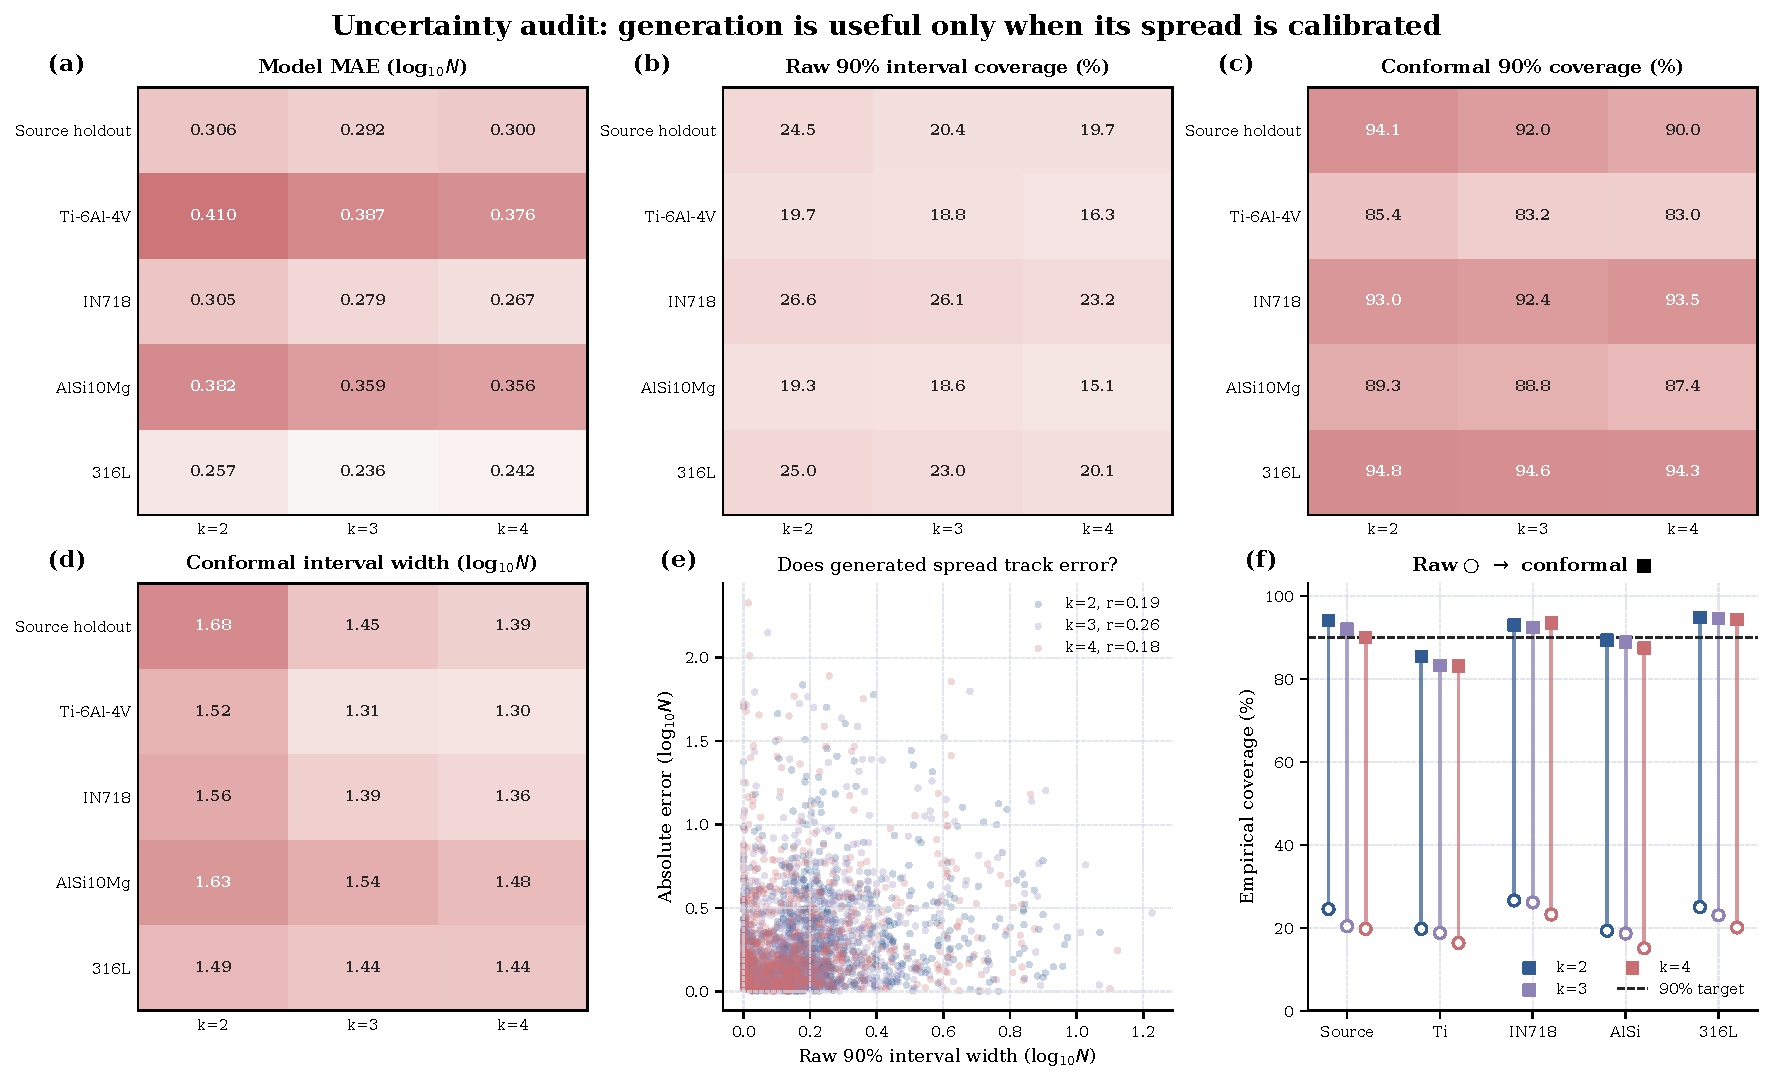
\includegraphics[width=\textwidth,height=0.38\textheight,keepaspectratio]{figs/uncertainty_audit.pdf}
\caption{\textbf{Question: Does stochastic spread behave as calibrated predictive uncertainty across strict splits?} Panels (a--d) compare point error, raw coverage, conformal coverage and calibrated width; panel (e) relates raw interval width to absolute error; panel (f) shows the change from raw to conformal coverage. \textbf{Finding:} generated spread contains a weak error signal but is substantially under-dispersed before calibration. Split-conformal expansion restores coverage toward its target, with residual shortfall under the strongest alloy shift.}
\label{fig:uncertainty_v2}
\end{figure*}

\subsection{Compared methods}

The main comparison spans three baseline families. Linear, polynomial and PCHIP interpolation test whether simple curve geometry is sufficient. $k$NN, random forest and ExtraTrees test conventional data-driven regression without a physical intermediate state. Direct U-Net tests deterministic deep completion with the same grid and input information. All methods receive the same held-out curves and hash-derived masks. Basquin-only and a matched bridge without the physical state remain component ablations because Basquin supplies the physical endpoint of the proposed method.

Hyperparameters for learned baselines are fixed before opening the test curves, using validation performance and the pre-declared settings released with the evaluation code. Direct U-Net uses the same grid representation and comparable channel width as the proposed backbone. Matched architecture and physics ablations use shared splits, masks and seeds; between-seed standard deviations and paired curve-bootstrap confidence intervals quantify their uncertainty.

\subsection{Evaluation metrics}

Hidden-point performance uses MAE, median absolute error and factor-of-two accuracy. Factor-of-two accuracy is the fraction with $|\hat y-y|\leq\log_{10}2$ and has a direct multiplicative-life interpretation. Full-grid evaluation uses mean absolute error against the reference interpolant, global log--log slope error and monotonicity-violation rate.

Probability quality uses CRPS for individual hidden points, WIS for central intervals, and Energy Score for the entire 32-dimensional curve. Variogram Score emphasizes dependence between stress locations. Calibration is reported as empirical coverage at 50\%, 80\%, 90\% and 95\%, mean width, absolute coverage error and simultaneous curve coverage. Average pairwise $L_1$ distance summarizes diversity, while proper scores determine distributional quality.

Statistical comparisons are paired by curve and mask. For each metric, 10,000 group-bootstrap replicates resample source papers. Improvements are assigned when the corresponding 95\% confidence interval excludes zero, and multiple comparisons across baselines use Holm correction. Database-resolved reporting gives AM2022, CMA2022 and Weld2025 independent visibility despite their different sizes.

\subsection{Expanded reconstruction benchmark}

The reported pooled test contains 789 untouched curves after validation-only gate fitting: 188 AM2022, 20 CMA2022 and 581 welded-joint curves. Table~\ref{tab:expanded_reconstruction} gives the aligned AM2022 comparison under six non-physics baselines. \method{} has the lowest full-grid error at all three sparse budgets. It leads seven of eight hidden-point metrics with two observations, six of eight with three observations and all eight with four observations; random forest or ExtraTrees leads the remaining RMSE and upper-tail-error cells.

\begin{table*}[t]
\caption{AM2022 source-paper-held-out comparison under identical sparse masks. The main comparison contains non-physics baselines; component variants are reported in the ablation study. Bold and underline mark first and second place.}
\label{tab:expanded_reconstruction}
\centering\scriptsize\setlength{\tabcolsep}{2.8pt}
\resizebox{\textwidth}{!}{%
\begin{tabular}{lrrrrrrrr}
\toprule
Method & MAE $\downarrow$ & RMSE $\downarrow$ & MedAE $\downarrow$ & P90AE $\downarrow$ & $R^2\uparrow$ & Pearson $r\uparrow$ & F2 $\uparrow$ & F3 $\uparrow$ \\
\midrule
\multicolumn{9}{c}{\textbf{$k=2$ observed tests}} \\
\midrule
kNN & 0.465 & 0.639 & 0.342 & 1.026 & 0.622 & 0.802 & 0.458 & 0.630 \\
RF & \underline{0.384} & \textbf{0.531} & \underline{0.275} & \underline{0.867} & \underline{0.738} & \underline{0.860} & \underline{0.536} & \underline{0.719} \\
ET & 0.391 & 0.537 & \underline{0.275} & 0.908 & 0.732 & 0.857 & 0.526 & 0.699 \\
Linear & 0.852 & 1.518 & 0.346 & 2.626 & -1.137 & 0.454 & 0.458 & 0.594 \\
Poly. & 0.845 & 1.507 & 0.346 & 2.599 & -1.105 & 0.457 & 0.458 & 0.595 \\
PCHIP & 0.852 & 1.518 & 0.346 & 2.626 & -1.137 & 0.454 & 0.458 & 0.594 \\
\textbf{S-PA-CBB (ours)} & \textbf{0.373} & \underline{0.535} & \textbf{0.247} & \textbf{0.866} & \textbf{0.761} & \textbf{0.873} & \textbf{0.558} & \textbf{0.726} \\
\midrule
\multicolumn{9}{c}{\textbf{$k=3$ observed tests}} \\
\midrule
kNN & 0.441 & 0.595 & 0.326 & 0.973 & 0.672 & 0.837 & 0.472 & 0.656 \\
RF & \underline{0.364} & \underline{0.512} & \underline{0.247} & \textbf{0.830} & 0.757 & 0.871 & \underline{0.562} & \underline{0.727} \\
ET & 0.370 & \textbf{0.508} & 0.267 & \underline{0.847} & \underline{0.761} & \underline{0.875} & 0.543 & 0.726 \\
Linear & 0.705 & 1.299 & 0.286 & 2.104 & -0.564 & 0.559 & 0.518 & 0.654 \\
Poly. & 0.914 & 1.608 & 0.352 & 2.860 & -1.396 & 0.433 & 0.456 & 0.580 \\
PCHIP & 1.005 & 1.749 & 0.360 & 3.463 & -1.835 & 0.401 & 0.445 & 0.571 \\
\textbf{S-PA-CBB (ours)} & \textbf{0.360} & 0.516 & \textbf{0.241} & 0.885 & \textbf{0.777} & \textbf{0.882} & \textbf{0.582} & \textbf{0.741} \\
\midrule
\multicolumn{9}{c}{\textbf{$k=4$ observed tests}} \\
\midrule
kNN & 0.424 & 0.566 & 0.319 & 0.928 & 0.710 & 0.853 & 0.479 & 0.672 \\
RF & \underline{0.374} & 0.529 & \underline{0.255} & 0.870 & 0.746 & 0.865 & \underline{0.561} & \underline{0.728} \\
ET & 0.382 & \underline{0.523} & 0.277 & \underline{0.865} & \underline{0.752} & \underline{0.868} & 0.532 & 0.703 \\
Linear & 0.605 & 1.154 & 0.257 & 1.395 & -0.208 & 0.631 & 0.550 & 0.683 \\
Poly. & 0.673 & 1.275 & 0.282 & 1.782 & -0.474 & 0.496 & 0.518 & 0.657 \\
PCHIP & 0.811 & 1.508 & 0.303 & 2.503 & -1.062 & 0.444 & 0.499 & 0.631 \\
\textbf{S-PA-CBB (ours)} & \textbf{0.321} & \textbf{0.468} & \textbf{0.207} & \textbf{0.743} & \textbf{0.817} & \textbf{0.904} & \textbf{0.625} & \textbf{0.771} \\
\bottomrule
\end{tabular}%
}
\end{table*}


Figure~\ref{fig:pooled_visuals} summarizes the promoted main model. It reports the validation gate, pooled complete-curve error against both the physical state and unconditional bridge, activation frequency and raw-versus-conformal calibration. Unlike a comparison based only on hidden points, it directly tests the quantity generated by the model: the complete curve.

\begin{figure*}[!t]
\centering
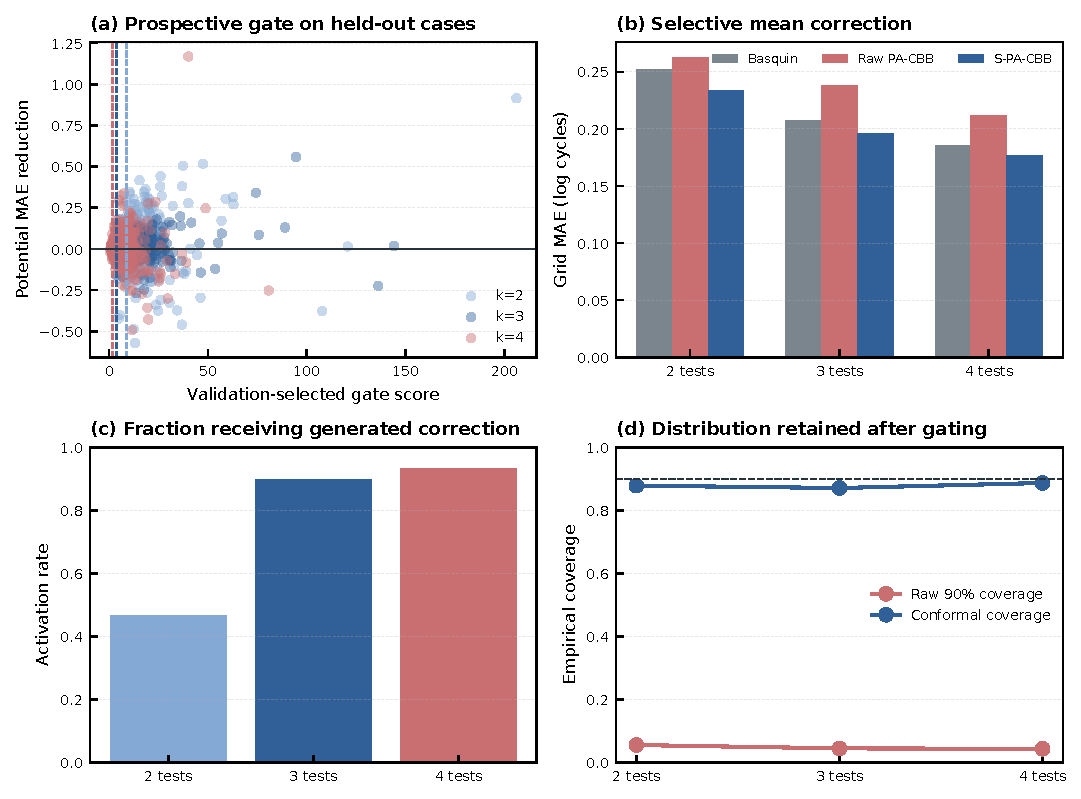
\includegraphics[width=0.98\textwidth,height=0.38\textheight,keepaspectratio]{figs/selective_main_overview.pdf}
\caption{\textbf{Question: Does the two-stage decision improve complete-curve reconstruction?} Panel (a) audits the Stage-I difficulty score; panel (b) compares retaining physics, transforming every curve and selectively transforming flagged curves; panel (c) reports the fraction assigned to the difficult class; panel (d) verifies that Stage II retains a distribution for calibration. \textbf{Finding:} the two-stage rule has the lowest pooled grid MAE for every sparse budget.}
\label{fig:pooled_visuals}
\end{figure*}

\subsection{Distributional evaluation and calibration}\label{sec:distributional}

For $k=2,3,4$, pooled CRPS is 0.292, 0.264 and 0.245, while Energy Score is 0.277, 0.236 and 0.213 under the frozen three-step sampler and selective mean translation. Energy Score is especially relevant because a sampled curve is evaluated as one 32-dimensional object.

The raw ensemble is sharply under-dispersed. Nominal 90\% intervals cover 5.6\%, 4.5\% and 4.4\% of hidden points. Validation-only split-conformal expansion raises coverage to 87.9\%, 87.2\% and 88.8\%, with mean interval widths of 1.302, 1.208 and 1.170 log cycles. These results identify the generated ensemble as the structured uncertainty carrier and conformal expansion as the coverage-control layer.

Figure~\ref{fig:curve_gallery} provides a qualitative success-case view across two, three and four revealed tests and the three principal databases. Thin trajectories and the 90\% band expose the generated distribution, while the reference, posterior mean and observed anchors locate its support. Cases are selected by a deterministic rule requiring low final grid error and, for activated cases, a positive correction gain; Table~\ref{tab:expanded_reconstruction} supplies the corresponding aggregate rather than case-selected evidence.

\begin{figure*}[!t]
\centering
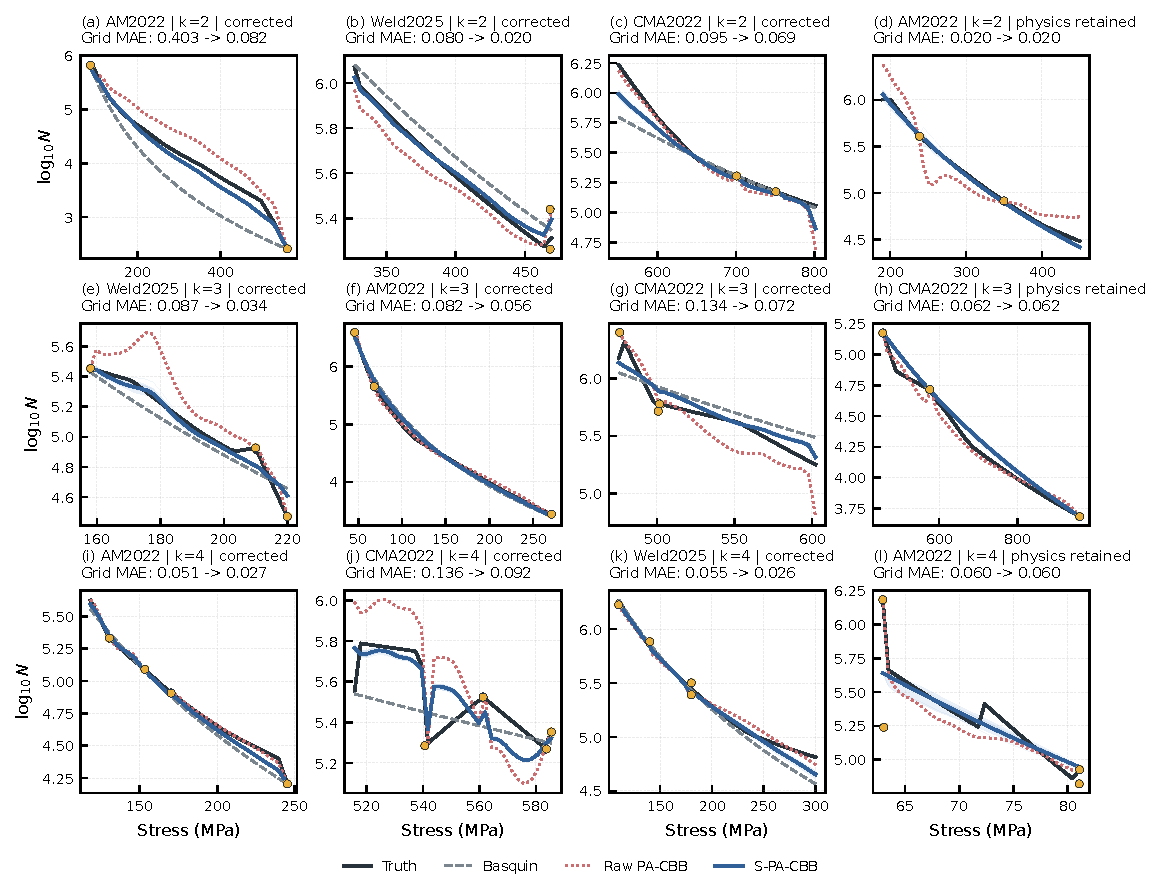
\includegraphics[width=0.98\textwidth,height=0.42\textheight,keepaspectratio]{figs/selective_curve_gallery.pdf}
\caption{\textbf{Question: Can selective conditional generation accurately reconstruct individual sparse S--N curves?} Twelve successful untouched pooled-test cases span $k=2,3,4$ and AM2022, CMA2022 and Weld2025. Each row contains three activated corrections and one accurate retained-physics case, selected by a fixed low-final-error, positive-gain rule. Curves show the reference, Basquin state, selective posterior mean, repeated trajectories, raw 90\% band and known anchors. \textbf{Finding:} accurate reconstructions arise through both targeted residual correction and appropriate retention of an already sufficient physical state.}
\label{fig:curve_gallery}
\end{figure*}

The gallery also exposes the action of the selective layer. Each sparse-budget row contains three gate-active examples whose blue mean departs from Basquin after validation evidence supports a residual correction, followed by one case in which the accurate sparse physical mean is retained while posterior trajectories are preserved. Both paths therefore produce decision-ready uncertainty, with the gate controlling the central transformation.

Across the gallery, observed anchors are re-imposed exactly after every reverse step. Differences between the selective mean and the reference therefore occur between or beyond measured stresses. The deliberately selected success cases illustrate attainable reconstruction quality and are not used to infer population performance; the aligned tables and pooled metrics establish the dataset-level trend.

The cases also show why the gate is budget-specific. With two observations, a large apparent residual can arise from an unstable physical slope as well as from genuine curvature, so the validation rule is conservative and accepts only half of the raw mean residual when activated. Three and four observations reveal more of the curve geometry; the fitted rule activates more frequently, but still shrinks the translation. This behaviour is visible in the retained examples, where additional anchors improve the Basquin state enough that an aggressive learned mean would add error even though the posterior contains plausible alternatives.

Gate scores, thresholds and shrinkage coefficients are fixed on validation data, and the displayed test labels serve retrospective coloring and error calculation. The same frozen rule is applied to every database. In the welded domain, where condition metadata and curve shapes differ from the additive-manufacturing development data, the gate reduces the cost of a poorly transported mean and exposes shifted cases through posterior spread.

The gallery separates mean correction from generative uncertainty. Translating every trajectory by the same gated vector preserves deviations about the ensemble mean and therefore preserves the learned correlation between stress locations. Fatigue-strength inversion, mission-spectrum damage and next-test acquisition consequently operate on complete samples for both gate outcomes.

\begin{figure*}[!t]
\centering
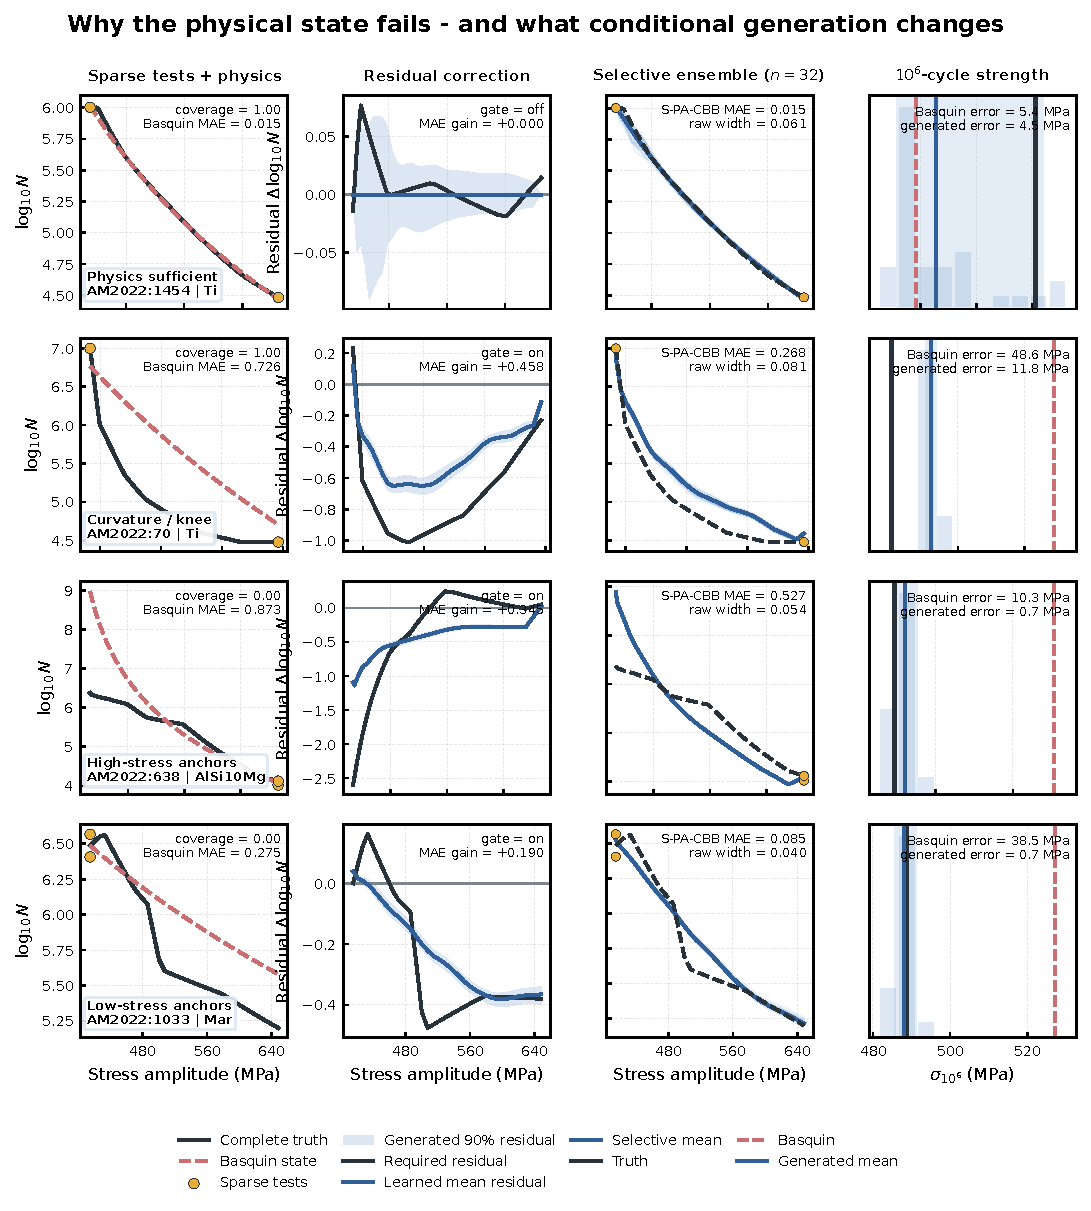
\includegraphics[width=0.95\textwidth,height=0.50\textheight,keepaspectratio]{figs/mechanism_case_studies.pdf}
\caption{\textbf{Question: Why does the sparse physical state fail, and what does selective generation change?} Each row is one held-out AM2022 curve from the pooled split. Columns show sparse observations and the Basquin state, required and selected generated residuals, 32 complete trajectories with their raw 90\% interval, and fatigue strength at $10^6$ cycles. The cases emphasize mechanism visibility. \textbf{Finding:} the gate retains a nearly single-slope curve, whereas curvature and one-sided extrapolation activate structured residuals that move an engineering quantity.}
\label{fig:mechanism_cases}
\end{figure*}

\subsection{What the generated residual changes}

The central interpretability question is which residual geometry the bridge learns beyond the physical state. Let
\begin{equation}
 \vect{r}^{\star}=\vect{y}_{\mathrm{true}}-\vect{y}_{\mathrm{phys}},
 \qquad
 \hat{\vect{r}}=\overline{\vect{y}}_{\method}-\vect{y}_{\mathrm{phys}},
 \label{eq:residual_audit}
\end{equation}
where $\vect{r}^{\star}$ is the correction required by the complete reference curve and $\hat{\vect{r}}$ is the correction learned by the posterior mean. This decomposition changes the interpretation of the experiment. Absolute prediction error asks whether the final curve is accurate; Eq.~\eqref{eq:residual_audit} asks what information the generator contributes beyond the sparse Basquin state.

Figure~\ref{fig:mechanism_cases} makes this decomposition concrete. The first, nearly single-slope Ti curve has Basquin grid MAE 0.015 log cycles; the gate remains off and the selective mean is unchanged. The curved Ti case activates a large stress-dependent residual: \method{} reduces grid MAE from 0.727 to 0.268 and the $10^6$-cycle fatigue-strength error from 48.6 to 11.8 MPa. The one-sided cases isolate extrapolation. With high-stress observations, the AlSi10Mg grid error falls from 0.873 to 0.528 and fatigue-strength error from 10.3 to 0.7 MPa. With low-stress observations, the maraging-steel curve falls from 0.275 to 0.085 log cycles and from 38.5 to 0.7 MPa. Together the cases show the mechanism directly: the gate suppresses unnecessary mean shifts and accepts residuals that coherently move a derived fatigue quantity.

The location and shape of this residual are engineering-relevant. A stress-dependent correction changes local slope and curvature, and hence changes fatigue-strength inversion, service-stress life, damage accumulation and the value of a future test at nearby stresses. The present data resolve these transitions at the curve level: the bridge targets observable departures from single-slope physics, and those departures alter the same functionals used in fatigue design. Mechanism-resolved fatigue records can connect these residual patterns to defect-controlled, microstructure-controlled and long-life regimes.

\begin{figure*}[!t]
\centering
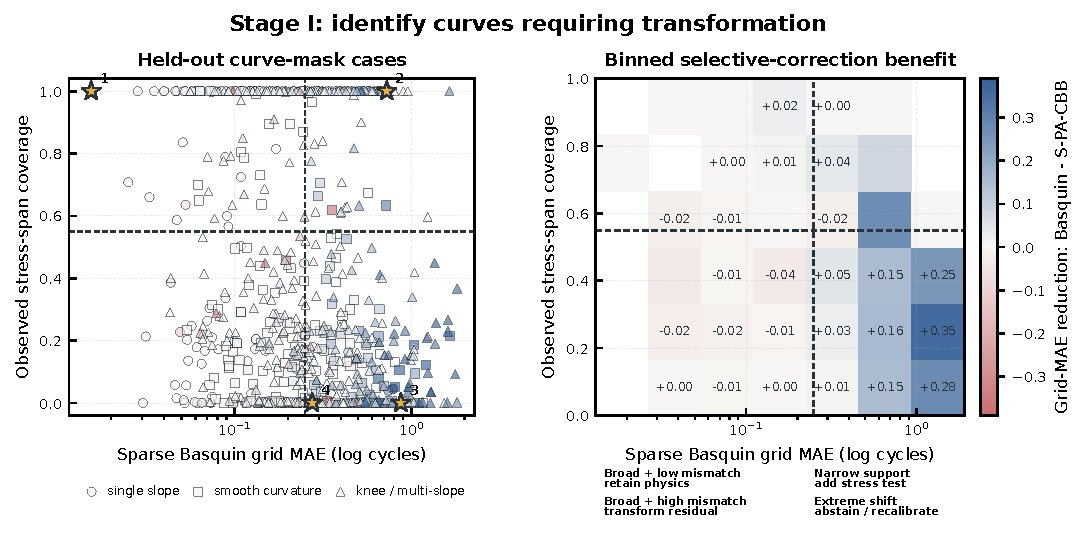
\includegraphics[width=0.98\textwidth,height=0.36\textheight,keepaspectratio]{figs/selective_use_mechanism_map.pdf}
\caption{\textbf{Which sparse curves require transformation?} Stage-I mechanism map for 752 held-out curve--mask cases. Basquin discrepancy, observed-span coverage and curve geometry separate physics-sufficient cases from high-mismatch cases that benefit from Stage-II transformation. Narrow support instead calls for another test or abstention. Stars locate Figure~\ref{fig:mechanism_cases}.}
\label{fig:selective_use_map}
\end{figure*}

Figure~\ref{fig:selective_use_map} audits the geometry that motivates Stage~I over all four sparse layouts. The validation-fitted difficulty screen leaves many physics-consistent cases unchanged, improves 27.5\% of all curve--mask cases and produces a positive mean reduction of 0.044 log cycles relative to Basquin. Broad support with small mismatch favours retention of the physical state. Broad support with a strong mismatch triggers Stage~II residual transformation. Narrow one-sided support prioritizes a separated stress level, while extreme shift activates calibrated abstention.

The horizontal coordinate is a retrospective visualization variable. Prospective inference uses the validation-calibrated generated-residual, support and spread proxies in Eq.~\eqref{eq:selective_gate}. The map therefore interprets the gate's operating regions, while the deployed rule remains fully prospective.

\begin{figure*}[!t]
\centering
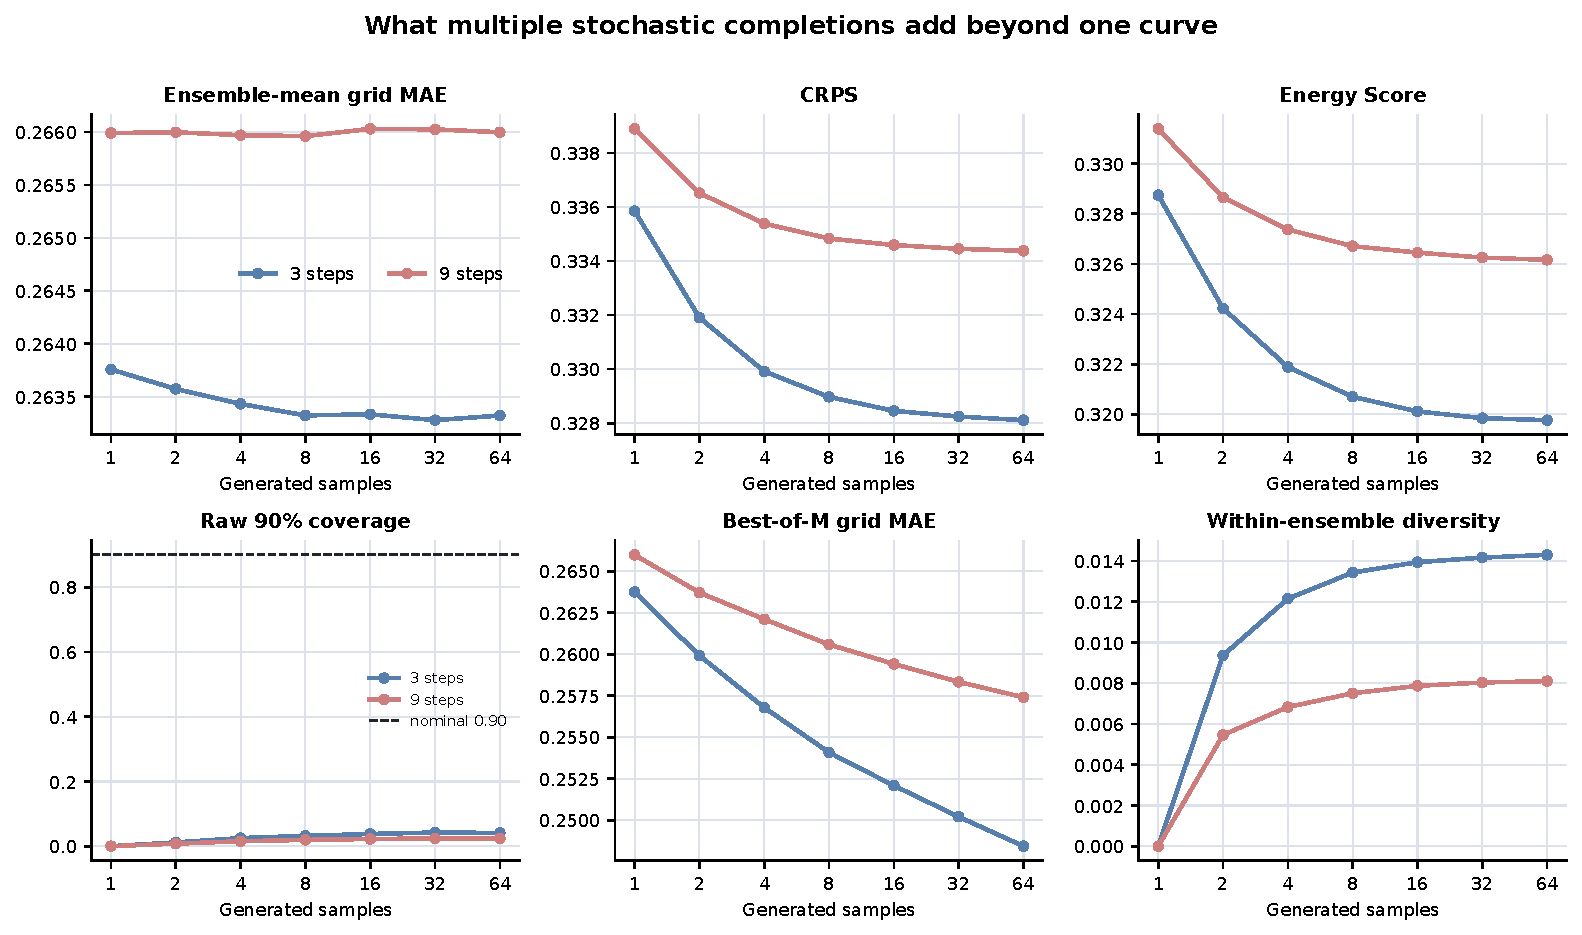
\includegraphics[width=0.98\textwidth,height=0.50\textheight,keepaspectratio]{figs/multiple_generation_value.pdf}
\caption{\textbf{Question: What is gained by drawing more than one conditional complete curve?} Results separate ensemble-mean accuracy, marginal and joint proper scores, raw coverage, oracle best-of-$M$ error and within-ensemble diversity for two reverse depths. \textbf{Finding:} the central prediction remains stable, whereas proper scores and representation of plausible alternatives improve before saturating. More samples expose distributional structure around the stable mean.}
\label{fig:multiple_generation_main}
\end{figure*}

\subsection{Why multiple generation is meaningful}

We test the value of stochastic generation by varying the number of curves while holding weights, sparse masks, transition scale and reverse-step schedule fixed. Figure~\ref{fig:multiple_generation_main} separates four effects. The ensemble-mean grid error is nearly invariant, whereas CRPS and Energy Score improve as more draws represent the empirical posterior, best-of-$M$ error decreases and within-ensemble diversity approaches a plateau. The useful change concentrates in the first 16--32 samples.

The transition-noise intervention supplies a causal check. At $\eta=0$, repeated calls collapse to the same trajectory. Increasing $\eta$ produces distinct curves and improves proper distributional scores while barely changing mean reconstruction error. The generated alternatives therefore carry conditional distributional information. Split-conformal calibration maps this structured but narrow spread to empirical coverage, and all decision results report raw spread and calibrated coverage separately.

Each draw is a coherent trajectory across stress, so its covariance propagates through inversion, integration and acquisition functions. The downstream active-learning experiment tests this property directly: multiple samples improve cross-stress covariance estimates until they stabilize. Distributional fidelity and reusable decision structure are therefore the two practical gains of generation.

\subsection{Ablation experiments}

The principal backbone check removes the physical endpoint while preserving the bridge, sampler, masks and training budget. Table~\ref{tab:core_ablation} labels this unconditional component as raw \rawmethod{}. Across the pooled test, the subsequent selective layer reduces grid MAE from 0.263 to 0.234, 0.239 to 0.196 and 0.212 to 0.176 for $k=2,3,4$, respectively. The table separately shows that the physical endpoint improves the raw generator. A noise intervention sets $\eta=0$: repeated curves collapse to one trajectory, whereas $\eta=0.5$ creates nonzero diversity and improves proper scores. Together these checks isolate the physical endpoint, stochastic transition and selective mean gate.

\begin{table}[t]
\caption{Backbone component checks before the selective gate. Values are means across the common three seeds; raw PA-CBB is the unconditional generative component of S-PA-CBB.}
\label{tab:core_ablation}
\centering\scriptsize\setlength{\tabcolsep}{4pt}
\begin{tabular}{lrrrr}
\toprule
Variant & $k$ & Grid MAE & Energy & Violation \\
\midrule
Raw PA-CBB & 2 & \textbf{0.287} & \textbf{0.343} & \textbf{0.160} \\
No physical state & 2 & 0.293 & 0.350 & 0.168 \\
Raw PA-CBB & 3 & \textbf{0.254} & \textbf{0.310} & \textbf{0.175} \\
No physical state & 3 & 0.263 & 0.320 & 0.182 \\
Raw PA-CBB & 4 & \textbf{0.233} & \textbf{0.286} & \textbf{0.179} \\
No physical state & 4 & 0.241 & 0.296 & 0.188 \\
\bottomrule
\end{tabular}
\end{table}


\iffalse

The completed campaign uses the three seeds shared by every learned variant (20261020--20261022). Restricting the table to this common intersection gives paired 3-versus-3 comparisons instead of mixing five runs for some variants with three for others. All variants share the source-paper split, sparse masks, three reverse steps, 32 draws and $\eta=0.5$. Relative to early concatenation, zero-initialized multi-scale control lowers grid MAE from 0.300 to 0.287 at $k=2$ and from 0.262 to 0.254 at $k=3$, with corresponding Energy Scores of 0.356 versus 0.343 and 0.315 versus 0.310. At $k=4$, early concatenation is marginally lower on both metrics. All paired curve-bootstrap intervals for these differences include zero. The aligned evidence therefore supports a sparsity-dependent trend, not a universal or statistically resolved ControlNet advantage. Parameter count does not explain the direction of the trend: the control model has 550,496 trainable parameters versus 710,549 for early concatenation.

The physical endpoint also improves the matched learned bridge on average: removing it increases mean grid MAE from 0.258 to 0.266 and Energy Score from 0.313 to 0.322. Paired intervals exclude zero at $k=3$ and $k=4$ but include zero at $k=2$; violation-rate differences exclude zero at every budget. Basquin-only, however, still has lower point and grid error and zero monotonicity violations on this source split. This negative result prevents claiming that learned stochastic corrections improve every point metric. Removing the first-difference loss leaves grid MAE and Energy Score nearly unchanged and slightly lowers slope error, but increases the average monotonicity-violation rate from 0.171 to 0.189; all three violation-rate intervals exclude zero. Thus the shape term is supported as a local physical-consistency regularizer rather than an accuracy term.

\begin{table*}[t]
\caption{Matched ablations on the fixed source-paper split under three reverse steps, 32 draws and $\eta=0.5$. Learned variants report mean $\pm$ between-seed standard deviation; Basquin is deterministic for a fixed mask.}
\label{tab:completed_ablation}
\centering
\scriptsize
\setlength{\tabcolsep}{3.5pt}
\begin{tabular}{lccccccc}
\toprule
Variant & $k$ & Seeds & Point MAE & Grid MAE & Slope error & Violation rate & Energy Score \\
\midrule
PA-CBB & 2 & 3 & 0.349 $\pm$ 0.005 & 0.287 $\pm$ 0.006 & 2.746 $\pm$ 0.116 & 0.160 $\pm$ 0.004 & 0.343 $\pm$ 0.005 \\
PA-CBB & 3 & 3 & 0.325 $\pm$ 0.009 & 0.254 $\pm$ 0.009 & 2.454 $\pm$ 0.055 & 0.175 $\pm$ 0.005 & 0.310 $\pm$ 0.011 \\
PA-CBB & 4 & 3 & 0.315 $\pm$ 0.011 & 0.233 $\pm$ 0.010 & 2.255 $\pm$ 0.084 & 0.179 $\pm$ 0.003 & 0.286 $\pm$ 0.012 \\
\addlinespace[2pt]
Early concat. & 2 & 3 & 0.362 $\pm$ 0.003 & 0.300 $\pm$ 0.002 & 2.937 $\pm$ 0.081 & 0.149 $\pm$ 0.003 & 0.356 $\pm$ 0.002 \\
Early concat. & 3 & 3 & 0.330 $\pm$ 0.004 & 0.262 $\pm$ 0.006 & 2.446 $\pm$ 0.157 & 0.170 $\pm$ 0.005 & 0.315 $\pm$ 0.007 \\
Early concat. & 4 & 3 & 0.311 $\pm$ 0.004 & 0.230 $\pm$ 0.006 & 2.308 $\pm$ 0.088 & 0.177 $\pm$ 0.004 & 0.283 $\pm$ 0.006 \\
\addlinespace[2pt]
No physics & 2 & 3 & 0.352 $\pm$ 0.002 & 0.293 $\pm$ 0.002 & 2.751 $\pm$ 0.036 & 0.168 $\pm$ 0.009 & 0.350 $\pm$ 0.002 \\
No physics & 3 & 3 & 0.328 $\pm$ 0.002 & 0.263 $\pm$ 0.001 & 2.436 $\pm$ 0.077 & 0.182 $\pm$ 0.006 & 0.320 $\pm$ 0.002 \\
No physics & 4 & 3 & 0.317 $\pm$ 0.005 & 0.241 $\pm$ 0.002 & 2.324 $\pm$ 0.024 & 0.188 $\pm$ 0.011 & 0.296 $\pm$ 0.003 \\
\addlinespace[2pt]
No shape loss & 2 & 3 & 0.350 $\pm$ 0.004 & 0.289 $\pm$ 0.003 & 2.665 $\pm$ 0.083 & 0.177 $\pm$ 0.004 & 0.345 $\pm$ 0.003 \\
No shape loss & 3 & 3 & 0.326 $\pm$ 0.005 & 0.254 $\pm$ 0.003 & 2.300 $\pm$ 0.077 & 0.194 $\pm$ 0.004 & 0.309 $\pm$ 0.003 \\
No shape loss & 4 & 3 & 0.316 $\pm$ 0.004 & 0.233 $\pm$ 0.003 & 2.190 $\pm$ 0.057 & 0.195 $\pm$ 0.007 & 0.286 $\pm$ 0.002 \\
\addlinespace[2pt]
Basquin only & 2 & 1 & 0.314 & 0.245 & 2.624 & 0.000 & -- \\
Basquin only & 3 & 1 & 0.283 & 0.206 & 2.226 & 0.000 & -- \\
Basquin only & 4 & 1 & 0.279 & 0.195 & 2.108 & 0.000 & -- \\
\bottomrule
\end{tabular}
\end{table*}


\begin{figure*}[t]
\centering
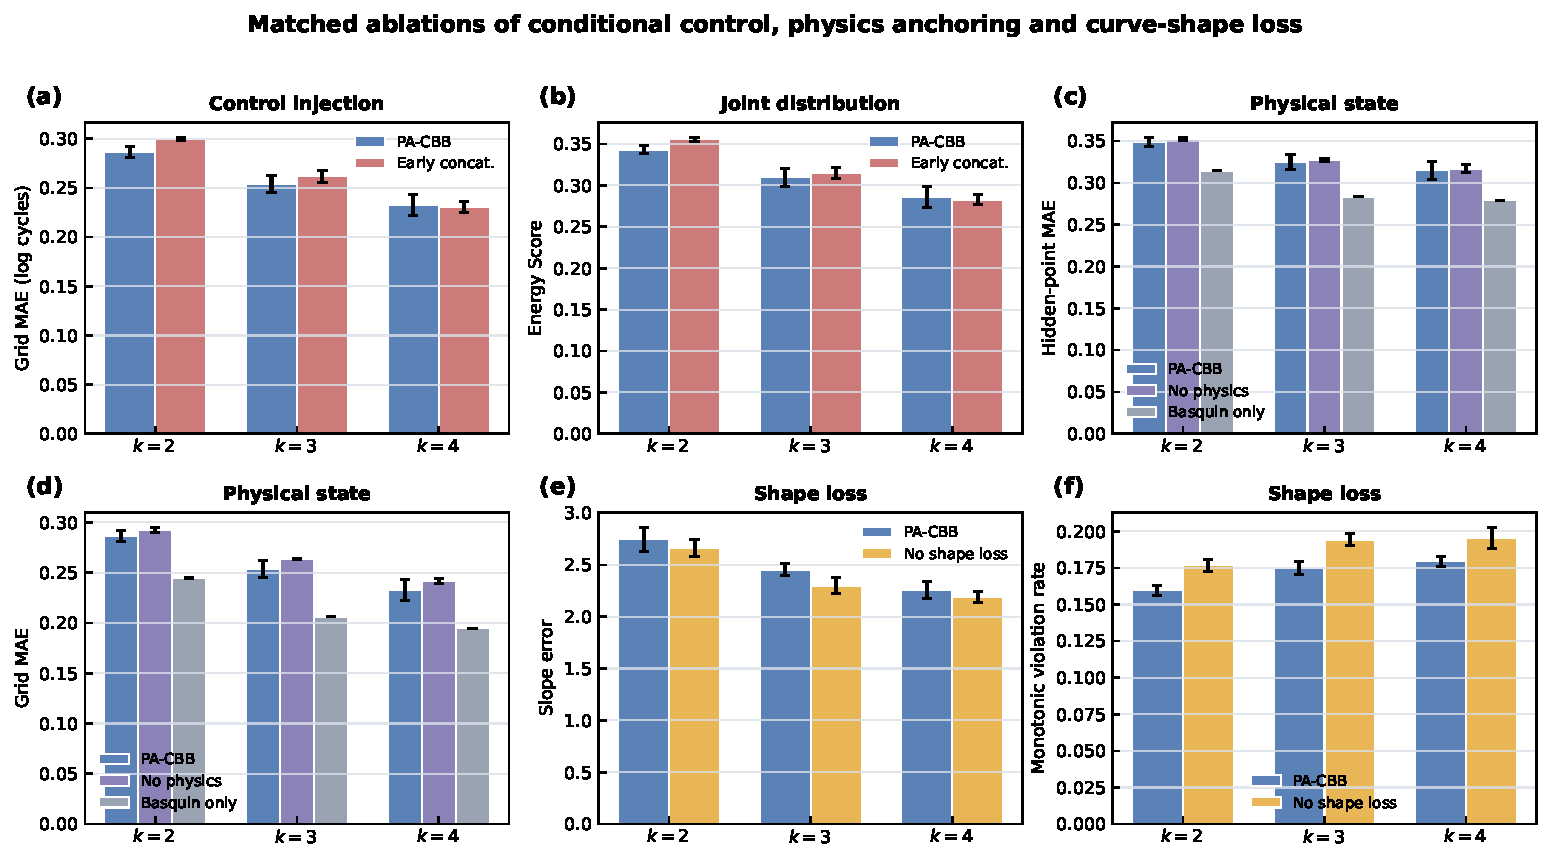
\includegraphics[width=\textwidth,height=0.40\textheight,keepaspectratio]{figs/completed_ablation.pdf}
\caption{\textbf{Question: Which components are necessary under one matched three-step protocol?} Bars show seed means and between-seed standard deviations. \textbf{Finding:} the physical endpoint consistently improves the learned bridge, the ControlNet-style path has an unresolved sparsity-dependent trend relative to early concatenation, Basquin remains the strongest deterministic point ablation, and the shape loss reduces monotonicity violations without improving mean error.}
\label{fig:ablation_v2}
\end{figure*}

\subsubsection{Physical-state shrinkage and monotone projection}

The fitted Basquin slope uses ridge shrinkage toward the training-set slope prior. Table~\ref{tab:shrinkage} varies only this ridge coefficient across five full-model seeds. With two observations, removing shrinkage raises grid MAE from 0.287 to 0.311, slope error from 2.55 to 2.68 and Energy Score from 0.341 to 0.367. Weak and current shrinkage are nearly tied, whereas strong shrinkage begins to increase error. At three and four observations the differences are small because the data dominate the prior. The benefit of physical shrinkage is therefore concentrated in the genuinely underdetermined two-point regime.

\begin{table*}[t]
\caption{Physical-slope shrinkage under the frozen three-step sampler. Values are mean $\pm$ standard deviation across five full-model seeds.}
\label{tab:shrinkage}
\centering\scriptsize\setlength{\tabcolsep}{5pt}
\begin{tabular}{lccccc}
\toprule
Variant & $k$ & Hidden MAE $\downarrow$ & Grid MAE $\downarrow$ & Slope error $\downarrow$ & Energy Score $\downarrow$ \\
\midrule
Current ($10^{-2}$) & 2 & 0.348 $\pm$ 0.003 & 0.287 $\pm$ 0.007 & 2.554 $\pm$ 0.116 & 0.341 $\pm$ 0.008 \\
Current ($10^{-2}$) & 3 & 0.315 $\pm$ 0.005 & 0.246 $\pm$ 0.007 & 2.371 $\pm$ 0.156 & 0.299 $\pm$ 0.009 \\
Current ($10^{-2}$) & 4 & 0.310 $\pm$ 0.003 & 0.230 $\pm$ 0.005 & 2.139 $\pm$ 0.093 & 0.281 $\pm$ 0.006 \\
No shrinkage & 2 & 0.376 $\pm$ 0.005 & 0.311 $\pm$ 0.010 & 2.678 $\pm$ 0.179 & 0.367 $\pm$ 0.011 \\
No shrinkage & 3 & 0.320 $\pm$ 0.003 & 0.250 $\pm$ 0.005 & 2.390 $\pm$ 0.174 & 0.303 $\pm$ 0.006 \\
No shrinkage & 4 & 0.308 $\pm$ 0.004 & 0.231 $\pm$ 0.005 & 2.107 $\pm$ 0.122 & 0.281 $\pm$ 0.006 \\
Strong ($10^{-1}$) & 2 & 0.353 $\pm$ 0.002 & 0.291 $\pm$ 0.006 & 2.594 $\pm$ 0.127 & 0.346 $\pm$ 0.007 \\
Strong ($10^{-1}$) & 3 & 0.316 $\pm$ 0.004 & 0.247 $\pm$ 0.007 & 2.384 $\pm$ 0.155 & 0.300 $\pm$ 0.008 \\
Strong ($10^{-1}$) & 4 & 0.310 $\pm$ 0.004 & 0.231 $\pm$ 0.005 & 2.161 $\pm$ 0.097 & 0.282 $\pm$ 0.006 \\
Weak ($10^{-3}$) & 2 & 0.347 $\pm$ 0.002 & 0.287 $\pm$ 0.006 & 2.514 $\pm$ 0.142 & 0.341 $\pm$ 0.007 \\
Weak ($10^{-3}$) & 3 & 0.318 $\pm$ 0.004 & 0.248 $\pm$ 0.006 & 2.384 $\pm$ 0.153 & 0.302 $\pm$ 0.007 \\
Weak ($10^{-3}$) & 4 & 0.308 $\pm$ 0.004 & 0.230 $\pm$ 0.004 & 2.128 $\pm$ 0.100 & 0.281 $\pm$ 0.006 \\
\bottomrule
\end{tabular}
\end{table*}


Table~\ref{tab:monotonicity} separates no shape loss, the deployed soft first-difference loss and a weighted hard isotonic projection. The hard projection eliminates all violations and lowers grid MAE to 0.253, 0.207 and 0.187 for $k=2,3,4$, respectively. This apparent gain is not free: projection moves the observed anchors by 0.013, 0.026 and 0.032 log cycles on average because noisy or repeated experimental anchors are not always jointly monotone. Exact anchor preservation and an everywhere-monotone curve can be mutually incompatible. We therefore retain the soft loss in the principal model and report hard projection as an optional decision-time operation rather than crediting it as an unconstrained model improvement.

\begin{table*}[t]
\caption{Monotonicity treatments on three common paired seeds. Hard projection is weighted toward observed anchors; anchor shift reports its mean absolute change at those anchors.}
\label{tab:monotonicity}
\centering\scriptsize\setlength{\tabcolsep}{4pt}
\begin{tabular}{lcccccc}
\toprule
Variant & $k$ & Grid MAE $\downarrow$ & Slope error $\downarrow$ & Violation rate $\downarrow$ & Energy Score $\downarrow$ & Anchor shift $\downarrow$ \\
\midrule
No shape loss & 2 & 0.289 $\pm$ 0.003 & 2.665 $\pm$ 0.083 & 0.177 $\pm$ 0.004 & 0.345 $\pm$ 0.003 & 0.000 $\pm$ 0.000 \\
No shape loss & 3 & 0.254 $\pm$ 0.003 & 2.300 $\pm$ 0.077 & 0.194 $\pm$ 0.004 & 0.309 $\pm$ 0.003 & 0.000 $\pm$ 0.000 \\
No shape loss & 4 & 0.233 $\pm$ 0.003 & 2.190 $\pm$ 0.057 & 0.195 $\pm$ 0.007 & 0.286 $\pm$ 0.002 & 0.000 $\pm$ 0.000 \\
Soft shape loss & 2 & 0.291 $\pm$ 0.004 & 2.601 $\pm$ 0.123 & 0.161 $\pm$ 0.002 & 0.345 $\pm$ 0.005 & 0.000 $\pm$ 0.000 \\
Soft shape loss & 3 & 0.248 $\pm$ 0.009 & 2.399 $\pm$ 0.206 & 0.170 $\pm$ 0.005 & 0.301 $\pm$ 0.011 & 0.000 $\pm$ 0.000 \\
Soft shape loss & 4 & 0.232 $\pm$ 0.005 & 2.163 $\pm$ 0.119 & 0.185 $\pm$ 0.001 & 0.283 $\pm$ 0.007 & 0.000 $\pm$ 0.000 \\
Hard monotone projection & 2 & 0.256 $\pm$ 0.002 & 2.531 $\pm$ 0.098 & 0.000 $\pm$ 0.000 & 0.315 $\pm$ 0.004 & 0.013 $\pm$ 0.000 \\
Hard monotone projection & 3 & 0.209 $\pm$ 0.005 & 2.186 $\pm$ 0.171 & 0.000 $\pm$ 0.000 & 0.264 $\pm$ 0.007 & 0.026 $\pm$ 0.000 \\
Hard monotone projection & 4 & 0.188 $\pm$ 0.003 & 1.924 $\pm$ 0.066 & 0.000 $\pm$ 0.000 & 0.240 $\pm$ 0.003 & 0.032 $\pm$ 0.000 \\
\bottomrule
\end{tabular}
\end{table*}


\begin{figure*}[t]
\centering
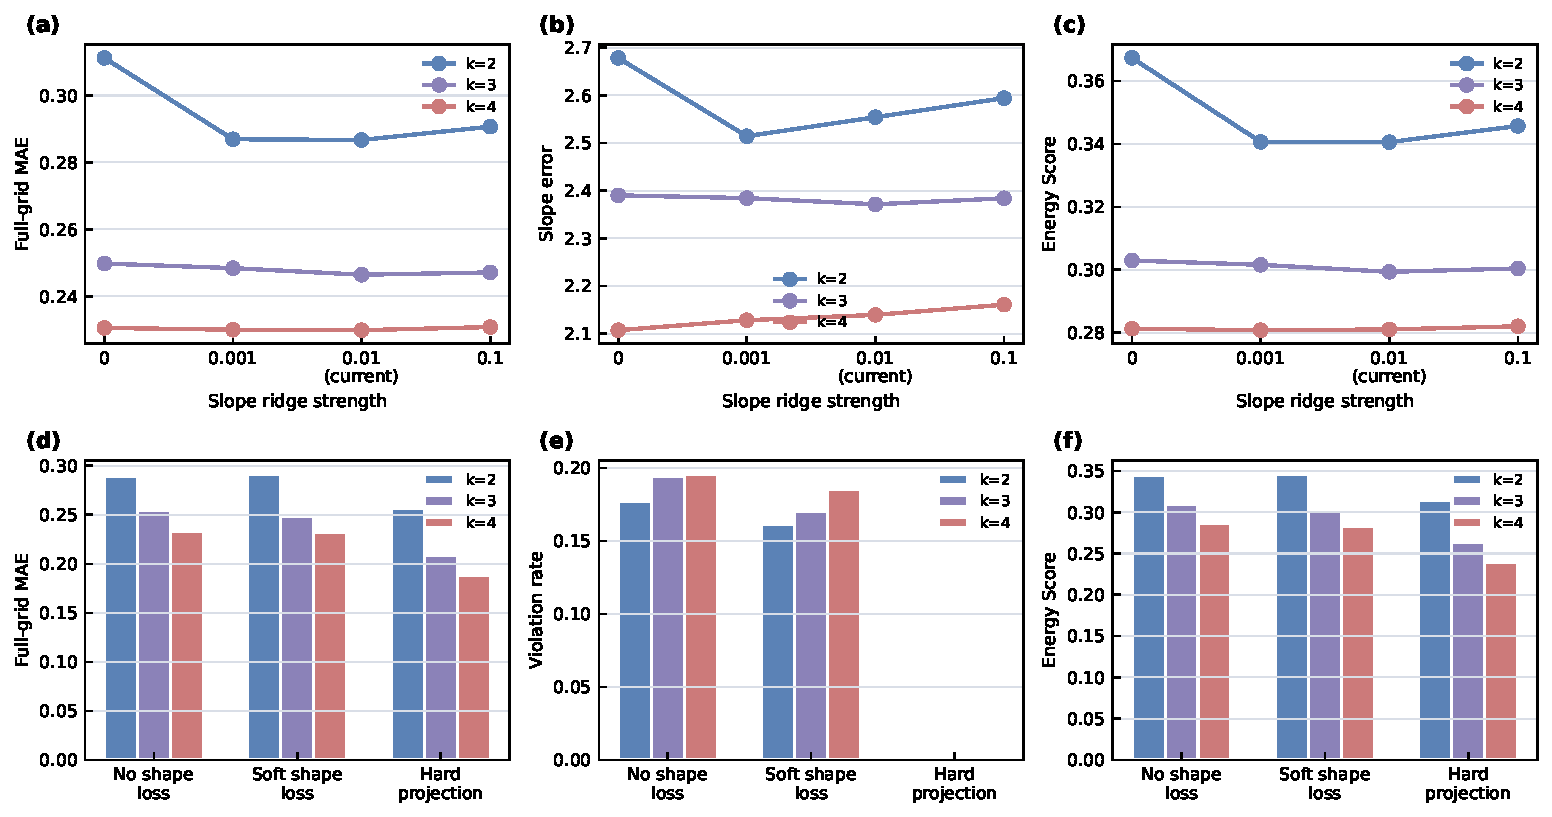
\includegraphics[width=\textwidth,height=0.43\textheight,keepaspectratio]{figs/physics_monotonicity_sensitivity.pdf}
\caption{\textbf{Question: How sensitive is the bridge to physical-slope shrinkage and monotonicity treatment?} The top row uses five full-model seeds; the bottom row uses the three common paired seeds. \textbf{Finding:} mild slope shrinkage is important primarily for two anchors. Hard projection improves average curve metrics and enforces zero violations, but it does so partly by moving measured anchors, so the soft loss remains the fidelity-preserving default.}
\label{fig:physics_monotonicity}
\end{figure*}

\subsubsection{Long-step and transition-noise audit}

The deployed sampler starts exactly at the physical endpoint, where Brownian-bridge variance is zero. For more than one reverse step it adds an independent Gaussian transition at every non-terminal state, $\eta\sqrt{t_{i+1}(1-t_{i+1})/K}\,\epsilon_i$. Thus the three-step main, external and downstream experiments are genuinely stochastic. The special one-step path has no intermediate state and is deterministic by construction; it must be interpreted as a point-prediction limit, not as a one-step generative model. We therefore reran the step ablation with exactly one output curve per condition, separating solver depth from Monte Carlo averaging.

\begin{table*}[t]
\caption{Single-sample long-step ablation. Time is synchronized accelerator inference time per curve.}
\label{tab:long_steps}
\centering\scriptsize
\begin{tabular}{rrrrrrr}
\toprule
Steps & Hidden MAE & Grid MAE & Energy & Slope error & Viol. rate & Time (s)\\
\midrule
1 & 0.329 & 0.259 & 0.323 & 2.488 & 0.189 & 0.0012\\
2 & 0.332 & 0.260 & 0.324 & 2.530 & 0.178 & 0.0015\\
3 & 0.336 & 0.264 & 0.329 & 2.583 & 0.172 & 0.0021\\
5 & 0.336 & 0.264 & 0.329 & 2.583 & 0.167 & 0.0033\\
9 & 0.339 & 0.266 & 0.331 & 2.608 & 0.163 & 0.0053\\
16 & 0.343 & 0.270 & 0.336 & 2.641 & 0.168 & 0.0087\\
32 & 0.345 & 0.272 & 0.338 & 2.681 & 0.170 & 0.0167\\
64 & 0.350 & 0.276 & 0.343 & 2.721 & 0.174 & 0.0328\\
128 & 0.352 & 0.278 & 0.345 & 2.760 & 0.173 & 0.0639\\
\bottomrule
\end{tabular}
\end{table*}

Figure~\ref{fig:long_steps} extends the sweep to 128 reverse steps. One step minimizes hidden-point MAE (0.329), grid MAE (0.259), Energy Score (0.324) and slope error (2.49). Three steps are the shortest genuinely stochastic configuration and retain most point accuracy, whereas 128 steps increase grid MAE to 0.278 and synchronized inference time from 0.0012 to 0.0639 s per curve. The result is not evidence that numerical refinement is intrinsically harmful. Diffusion sampling contains initialization, truncation, discretization and score-approximation errors~\cite{Pierret2025DiffusionErrors}; in this direct-$x_0$ first-order sampler, each additional transition re-evaluates an imperfect learned denoiser on its own previous output and injects fresh noise. Approximation errors can therefore accumulate faster than the discretization benefit. Dedicated high-order solvers are explicitly designed to avoid this trade-off and can reach strong diffusion samples in roughly 10--20 function evaluations~\cite{Lu2022DPMSolver}. For the present low-dimensional smooth-curve problem, three steps are the recommended generative default; one step is retained only when a deterministic point estimate is sufficient.

\begin{figure*}[t]
\centering
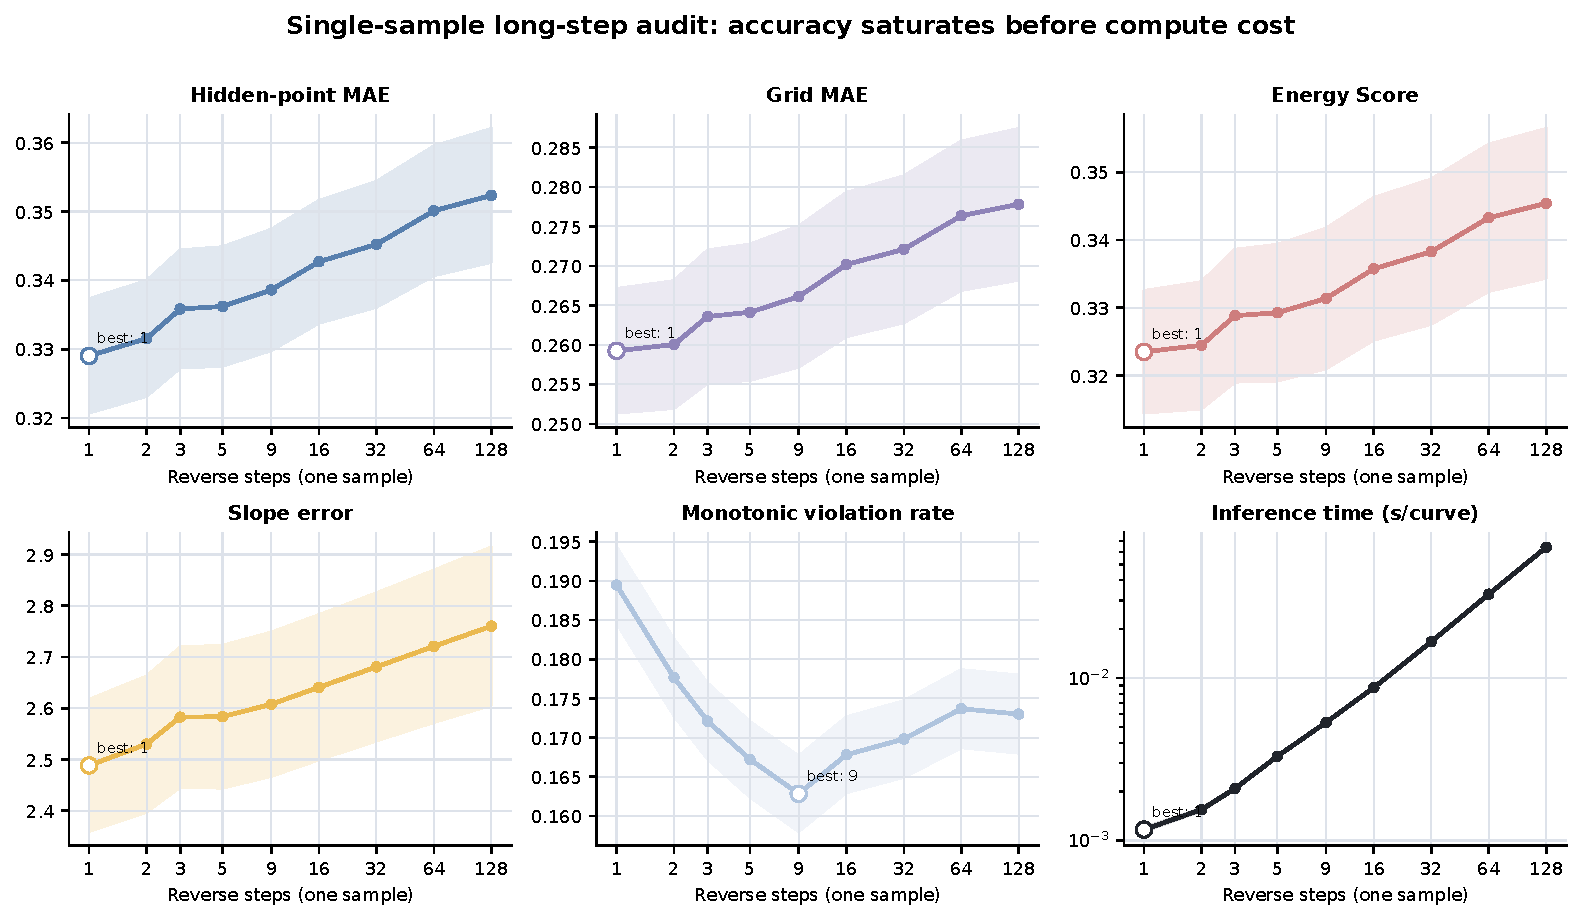
\includegraphics[width=\textwidth,height=0.43\textheight,keepaspectratio]{figs/long_step_single_sample.pdf}
\caption{\textbf{Question: Does a longer reverse trajectory improve one generated curve?} Every condition contributes one output, so the comparison is not aided by ensemble averaging. Shading denotes one standard error across held-out curve--mask cases. \textbf{Finding:} point and curve errors are lowest at one step, monotonicity is best near nine steps, and latency grows almost linearly through 128 steps.}
\label{fig:long_steps}
\end{figure*}

\subsubsection{Why stochastic generation is useful}

Generation is useful only if repeated samples improve distributional or decision quantities that a single curve cannot provide. Figure~\ref{fig:multiple_generation} tests this directly at three and nine steps. At three steps, increasing the ensemble from one to 64 leaves the ensemble-mean grid MAE essentially unchanged (0.264) but lowers CRPS from 0.336 to 0.328 and Energy Score from 0.329 to 0.320. Best-of-$M$ grid MAE falls from 0.264 to 0.248, demonstrating that the samples explore plausible alternatives around the mean rather than returning numerical duplicates. Most proper-score improvement is obtained by 16--32 samples. The best-of-$M$ metric is reported only as a diversity diagnostic because it uses the reference to select a sample and is not available prospectively.

The noise-scale intervention provides the causal check. With $\eta=0$, all 32 trajectories collapse to one curve, interval width and coverage are zero, and CRPS is 0.335. Raising $\eta$ to 1.0 changes grid MAE by only 0.0013 but improves CRPS to 0.322 and Energy Score from 0.328 to 0.313 while creating nonzero within-ensemble diversity. Therefore the stochastic term contributes useful conditional distributional information rather than improving the mean by repeated averaging. Raw 90\% coverage reaches only 8.4\%, however, so stochastic diversity is meaningful but under-dispersed; conformal calibration remains necessary. This distinction prevents equating ``many different curves'' with calibrated uncertainty.

\begin{figure*}[t]
\centering
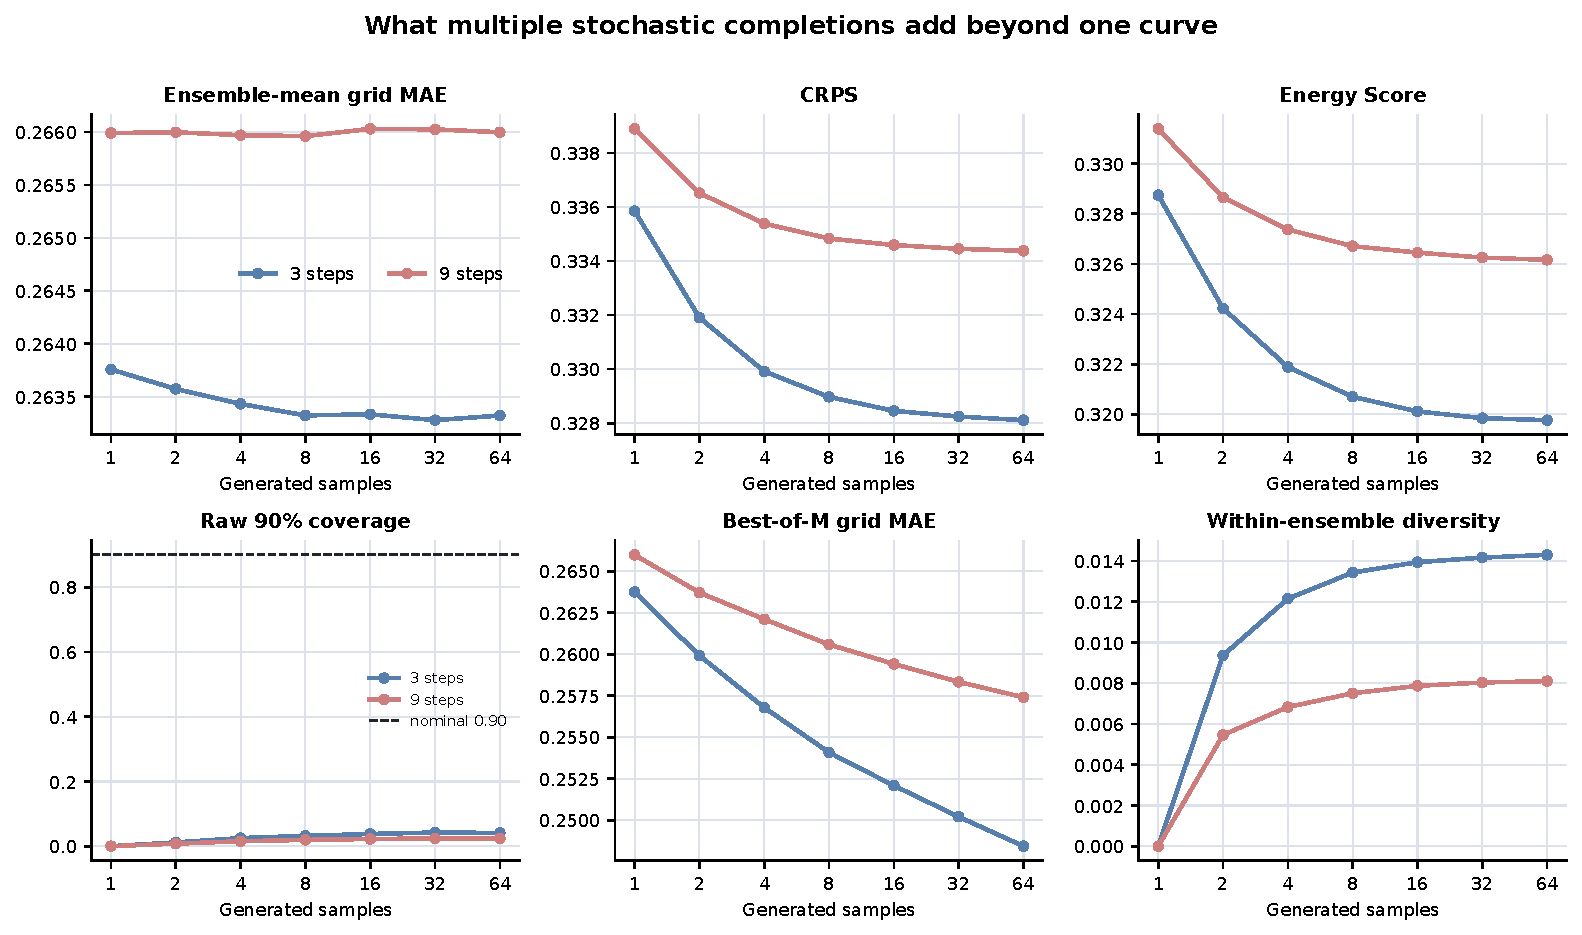
\includegraphics[width=\textwidth,height=0.60\textheight,keepaspectratio]{figs/multiple_generation_value.pdf}
\caption{\textbf{Question: What is gained by drawing more than one conditional curve?} \textbf{Finding:} ensemble-mean MAE is nearly invariant, whereas CRPS, Energy Score and best-of-$M$ error improve and diversity saturates near 16--32 samples. Three reverse steps dominate nine at equal ensemble size.}
\label{fig:multiple_generation}
\end{figure*}

The sweep separates three choices that are often conflated: reverse depth controls repeated network evaluation, ensemble size controls Monte Carlo approximation and $\eta$ controls stochastic spread. The evidence supports three reverse steps and 16--32 samples as the efficient generative setting. Calibration is then fitted to this fixed sampler; changing the step count or noise scale after calibration would define a different predictive procedure.

\begin{table*}[t]
\caption{Transition-noise ablation at three reverse steps and 32 generated curves.}
\label{tab:noise_ablation}
\centering\scriptsize
\begin{tabular}{rrrrrrrr}
\toprule
$\eta$ & Grid MAE & CRPS & Energy & Coverage & Width & Diversity & Time (s)\\
\midrule
0.00 & 0.263 & 0.335 & 0.328 & 0.000 & 0.000 & 0.000 & 0.0028\\
0.25 & 0.263 & 0.332 & 0.324 & 0.020 & 0.021 & 0.007 & 0.0023\\
0.50 & 0.263 & 0.328 & 0.320 & 0.045 & 0.042 & 0.014 & 0.0024\\
0.75 & 0.263 & 0.325 & 0.316 & 0.064 & 0.063 & 0.021 & 0.0021\\
1.00 & 0.264 & 0.322 & 0.313 & 0.084 & 0.085 & 0.029 & 0.0023\\
\bottomrule
\end{tabular}
\end{table*}
\begin{figure*}[t]
\centering
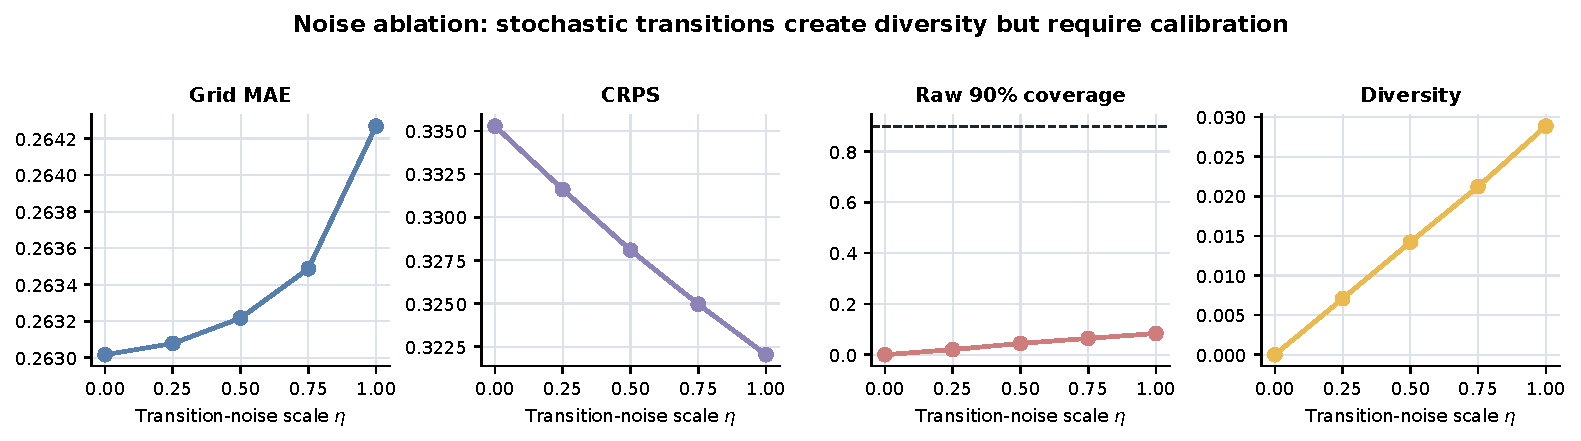
\includegraphics[width=\textwidth,height=0.25\textheight,keepaspectratio]{figs/noise_scale_ablation.pdf}
\caption{\textbf{Question: Are the repeated completions caused by an operative stochastic transition?} The experiment varies only $\eta$ at three steps and 32 samples. \textbf{Finding:} larger noise leaves the mean error nearly unchanged but improves proper scores and increases diversity; raw coverage remains far below nominal.}
\label{fig:noise_ablation}
\end{figure*}

\subsubsection{What the bridge adds to the physical state}

Figure~\ref{fig:residual_decomposition} decomposes the complete prediction into the Basquin state plus the learned bridge correction. The required correction is $y_{\mathrm{true}}-y_{\mathrm{Basquin}}$, and the learned correction is $\bar y_{\mathrm{PA-CBB}}-y_{\mathrm{Basquin}}$. Their pointwise correlation is 0.363, showing that the bridge learns a real residual direction, but its average correction is too aggressive on already accurate Basquin curves. Consequently, Basquin has lower overall grid MAE and the bridge improves only 38--39\% of all curves. The behavior changes in the regime for which a learned correction is most relevant: in the hardest Basquin-error quintile, PA-CBB reduces grid MAE by 0.070 on average and improves 69.7\% of curves; in the hardest decile, the reduction is 0.140 and 80.3\% of curves improve. Ensemble spread is also positively associated with difficult cases. The bridge therefore adds a failure-sensitive residual distribution, not a universal replacement for the physical law. This is the practically relevant role for screening: retain Basquin when it already fits, and use the generated correction and its calibrated uncertainty to flag conditions where sparse physics is unreliable.

\begin{figure*}[t]
\centering
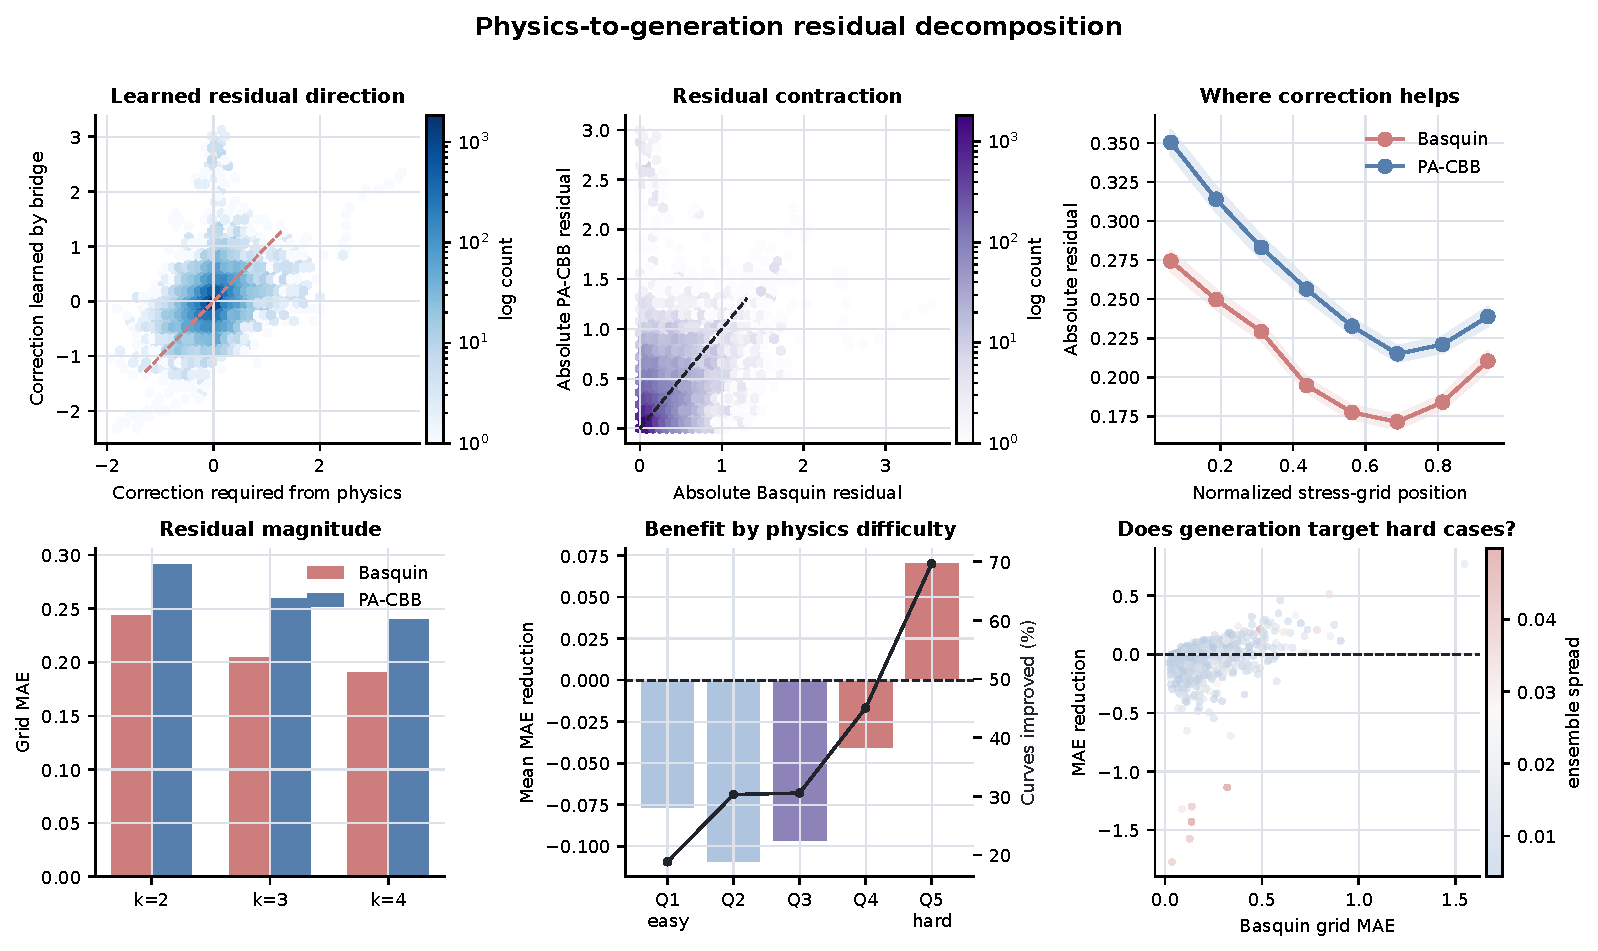
\includegraphics[width=\textwidth,height=0.60\textheight,keepaspectratio]{figs/physics_generation_residuals.pdf}
\caption{\textbf{Question: What does the Brownian bridge add beyond the Basquin state?} Residuals and corrections are evaluated on the complete 32-point grid. \textbf{Finding:} the bridge is worse on many easy physics cases but increasingly helpful as Basquin error grows, improving about 70\% of the hardest quintile and 80\% of the hardest decile.}
\label{fig:residual_decomposition}
\end{figure*}

\subsubsection{Robustness to sparse-point location}

Random masks do not represent every laboratory campaign. We therefore evaluate six deterministic or hash-randomized layouts under the same full checkpoints: random anchors, evenly spaced interior anchors, anchors concentrated at the high- or low-stress end, a contiguous center cluster and a layout spanning both endpoints. Interpolation and extrapolation are defined relative to the observed stress span, not the global grid.

Table~\ref{tab:mask_robustness} and Figure~\ref{fig:mask_robustness} show that coverage of the stress span matters more than the raw number of anchors. For three and four observations, endpoint-spanning layouts give the lowest hidden-point MAE (0.297 and 0.270) and Energy Score (0.293 and 0.268). High-stress-only masks have extrapolation MAE of 0.389, 0.374 and 0.383, while low-stress-only masks reach Energy Scores of 0.373, 0.346 and 0.319. Their within-span interpolation errors can look deceptively small because few hidden points lie inside the narrow observed range. Adjacent center points are also consistently worse than layouts covering the domain. The result quantifies a practical limitation of two-point Basquin conditioning: adding a well-separated stress level is more informative than adding another replicate near the same stress.

\begin{table*}[t]
\caption{Sparse-anchor location robustness across five full-model seeds. Interpolation and extrapolation are defined relative to the observed stress span; endpoint masks have no extrapolation points.}
\label{tab:mask_robustness}
\centering\scriptsize\setlength{\tabcolsep}{4pt}
\begin{tabular}{lcccccc}
\toprule
Mask pattern & $k$ & Hidden MAE $\downarrow$ & Interpolation MAE $\downarrow$ & Extrapolation MAE $\downarrow$ & Grid MAE $\downarrow$ & Energy Score $\downarrow$ \\
\midrule
Adjacent center & 2 & 0.361 $\pm$ 0.007 & 0.283 $\pm$ 0.009 & 0.363 $\pm$ 0.007 & 0.285 $\pm$ 0.006 & 0.341 $\pm$ 0.006 \\
Adjacent center & 3 & 0.355 $\pm$ 0.005 & 0.258 $\pm$ 0.004 & 0.356 $\pm$ 0.006 & 0.263 $\pm$ 0.006 & 0.321 $\pm$ 0.007 \\
Adjacent center & 4 & 0.341 $\pm$ 0.009 & 0.288 $\pm$ 0.004 & 0.345 $\pm$ 0.009 & 0.240 $\pm$ 0.007 & 0.296 $\pm$ 0.009 \\
Endpoints & 2 & 0.345 $\pm$ 0.006 & 0.345 $\pm$ 0.006 & -- & 0.293 $\pm$ 0.008 & 0.346 $\pm$ 0.009 \\
Endpoints & 3 & 0.297 $\pm$ 0.005 & 0.297 $\pm$ 0.005 & -- & 0.241 $\pm$ 0.008 & 0.293 $\pm$ 0.009 \\
Endpoints & 4 & 0.270 $\pm$ 0.004 & 0.270 $\pm$ 0.004 & -- & 0.217 $\pm$ 0.006 & 0.268 $\pm$ 0.007 \\
High-stress end & 2 & 0.387 $\pm$ 0.015 & 0.212 $\pm$ 0.004 & 0.389 $\pm$ 0.015 & 0.296 $\pm$ 0.011 & 0.357 $\pm$ 0.013 \\
High-stress end & 3 & 0.372 $\pm$ 0.014 & 0.125 $\pm$ 0.005 & 0.374 $\pm$ 0.014 & 0.261 $\pm$ 0.008 & 0.322 $\pm$ 0.009 \\
High-stress end & 4 & 0.379 $\pm$ 0.011 & 0.221 $\pm$ 0.013 & 0.383 $\pm$ 0.011 & 0.243 $\pm$ 0.007 & 0.303 $\pm$ 0.008 \\
Low-stress end & 2 & 0.387 $\pm$ 0.003 & 0.287 $\pm$ 0.005 & 0.387 $\pm$ 0.003 & 0.324 $\pm$ 0.005 & 0.373 $\pm$ 0.005 \\
Low-stress end & 3 & 0.368 $\pm$ 0.005 & 0.170 $\pm$ 0.015 & 0.369 $\pm$ 0.005 & 0.296 $\pm$ 0.005 & 0.346 $\pm$ 0.005 \\
Low-stress end & 4 & 0.348 $\pm$ 0.006 & 0.210 $\pm$ 0.015 & 0.350 $\pm$ 0.007 & 0.269 $\pm$ 0.007 & 0.319 $\pm$ 0.009 \\
Random & 2 & 0.348 $\pm$ 0.003 & 0.271 $\pm$ 0.007 & 0.373 $\pm$ 0.006 & 0.287 $\pm$ 0.007 & 0.341 $\pm$ 0.008 \\
Random & 3 & 0.315 $\pm$ 0.005 & 0.283 $\pm$ 0.003 & 0.344 $\pm$ 0.010 & 0.246 $\pm$ 0.007 & 0.299 $\pm$ 0.009 \\
Random & 4 & 0.310 $\pm$ 0.003 & 0.280 $\pm$ 0.003 & 0.363 $\pm$ 0.007 & 0.230 $\pm$ 0.005 & 0.281 $\pm$ 0.006 \\
Uniform interior & 2 & 0.343 $\pm$ 0.004 & 0.268 $\pm$ 0.002 & 0.365 $\pm$ 0.005 & 0.269 $\pm$ 0.003 & 0.326 $\pm$ 0.004 \\
Uniform interior & 3 & 0.325 $\pm$ 0.007 & 0.282 $\pm$ 0.004 & 0.352 $\pm$ 0.012 & 0.244 $\pm$ 0.006 & 0.302 $\pm$ 0.008 \\
Uniform interior & 4 & 0.311 $\pm$ 0.006 & 0.256 $\pm$ 0.004 & 0.338 $\pm$ 0.008 & 0.228 $\pm$ 0.007 & 0.281 $\pm$ 0.008 \\
\bottomrule
\end{tabular}
\end{table*}


\begin{figure*}[t]
\centering
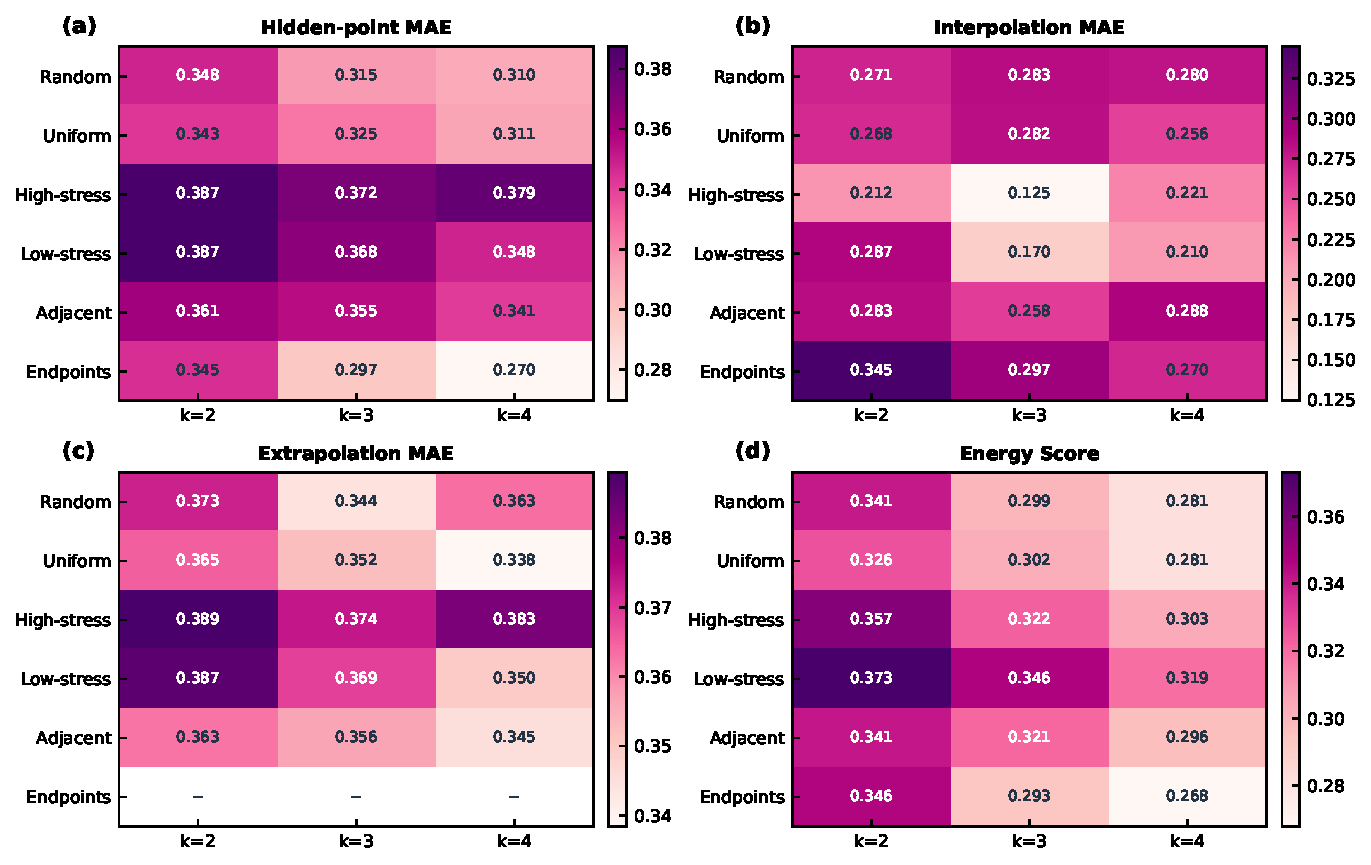
\includegraphics[width=\textwidth,height=0.45\textheight,keepaspectratio]{figs/mask_location_robustness.pdf}
\caption{\textbf{Question: Does performance depend on where the sparse fatigue tests are placed?} Values are means over five full-model seeds. Endpoint layouts have no extrapolation stratum because the observed span covers the grid. \textbf{Finding:} endpoint coverage is strongest for three and four anchors, while one-sided and adjacent clusters expose substantially larger extrapolation error.}
\label{fig:mask_robustness}
\end{figure*}

\fi

\subsection{Database-resolved pooled evaluation}

The final cross-database comparison fixes the three-step sampler, 32 generated curves, $\eta=0.5$ and one hash-derived sparse mask per curve. The same masks are used by every method. Stage-I gates and Stage-II correction strengths are selected on validation curves, and the test partitions are opened after these choices are frozen. The reported test set contains 188 AM2022, 20 CMA2022 and 581 Weld2025 curves. The comparison set comprises $k$NN, random forest, ExtraTrees, linear interpolation, polynomial interpolation and PCHIP; each cell is evaluated against its lowest-error member.

\begin{table*}[t]
\centering
\small
\setlength{\tabcolsep}{4.2pt}
\caption{Mask-aligned three-database evaluation. Point MAE is evaluated only at hidden measurements; grid MAE evaluates complete-curve reconstruction.}
\label{tab:three_database_latest}
\begin{tabular}{llrrrrrr}
\toprule
Database & $k$ & Curves & S-PA-CBB & Best non-physics & Gain (\%) & Grid MAE & Raw PA-CBB \\
\midrule
AM2022 & 2 & 188 & 0.370 & ET: 0.402 & +7.9 & 0.269 & 0.297 \\
AM2022 & 3 & 188 & 0.340 & RF: 0.386 & +12.0 & 0.243 & 0.278 \\
AM2022 & 4 & 188 & 0.326 & ET: 0.382 & +14.5 & 0.218 & 0.243 \\
CMA2022 & 2 & 20 & 0.424 & RF: 0.445 & +4.7 & 0.323 & 0.357 \\
CMA2022 & 3 & 20 & 0.371 & RF: 0.404 & +8.1 & 0.260 & 0.319 \\
CMA2022 & 4 & 20 & 0.418 & ET: 0.495 & +15.4 & 0.277 & 0.314 \\
Weld2025 & 2 & 581 & 0.282 & ET: 0.338 & +16.6 & 0.205 & 0.243 \\
Weld2025 & 3 & 581 & 0.267 & ET: 0.314 & +15.0 & 0.180 & 0.217 \\
Weld2025 & 4 & 581 & 0.253 & ET: 0.303 & +16.3 & 0.156 & 0.200 \\
\bottomrule
\end{tabular}
\begin{minipage}{0.98\textwidth}\footnotesize Comparator set: $k$NN, RF, ET, linear interpolation, polynomial interpolation and PCHIP. Gates and correction weights are selected exclusively on validation curves.\end{minipage}
\end{table*}


The selective model has lower hidden-point MAE than the strongest non-physics comparator in all nine database--budget cells. The relative reduction is 7.9--14.5\% for AM2022, 4.7--15.4\% for CMA2022 and 15.0--16.6\% for Weld2025. Residual shrinkage is central to these gains. At four observations, selective correction reduces raw-bridge grid MAE from 0.243 to 0.218 in AM2022, from 0.314 to 0.277 in CMA2022 and from 0.200 to 0.156 in Weld2025. The corresponding values are also below the sparse Basquin grid errors in all three reported databases.

\begin{figure*}[t]
\centering
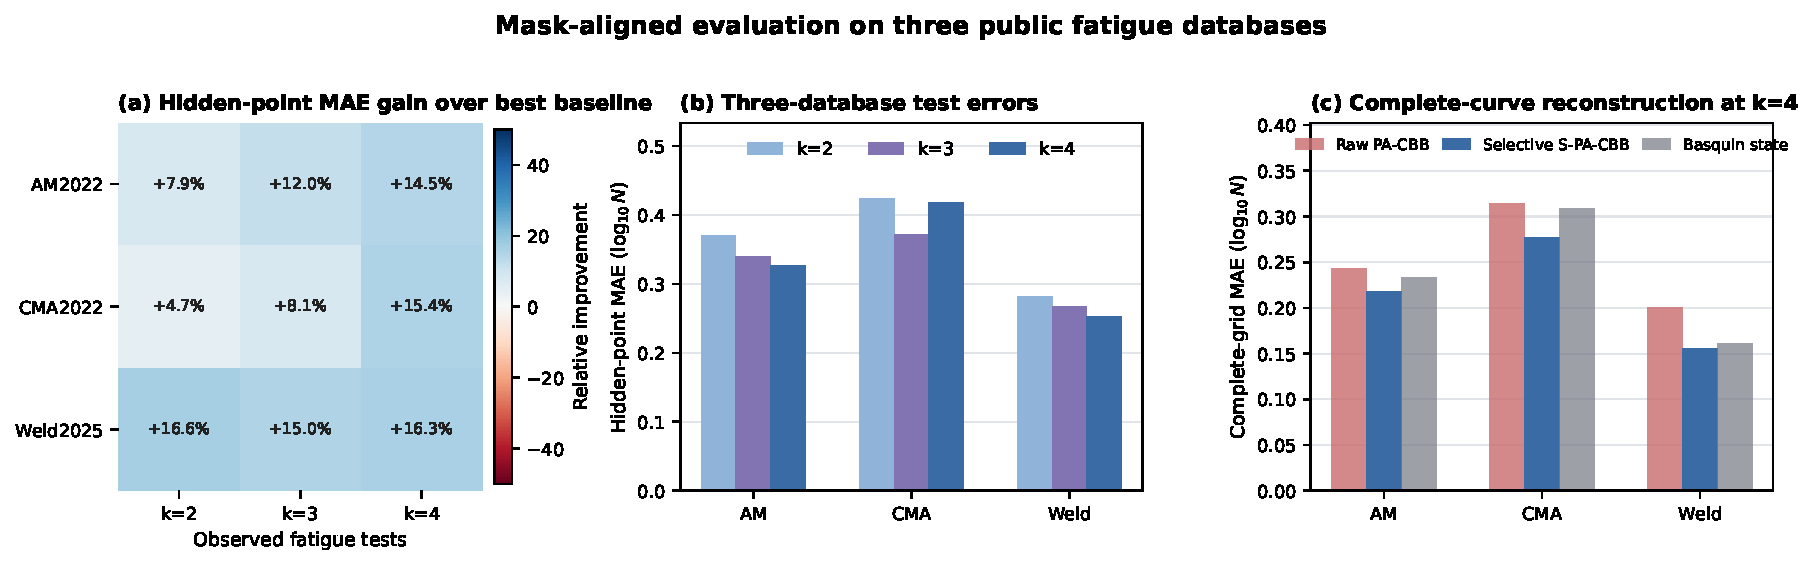
\includegraphics[width=\textwidth,height=0.32\textheight,keepaspectratio]{figs/three_database_latest_comparison.pdf}
\caption{\textbf{Question: Does validation-selected selective correction remain useful across the three reported databases?} Panel (a) gives the hidden-point MAE reduction relative to the strongest prespecified non-physics comparator; panel (b) reports absolute hidden-point error; panel (c) separates the raw generator, selective correction and Basquin state at four observations. \textbf{Finding:} \method{} leads all nine hidden-point comparisons, while the gate consistently shrinks the complete-grid error of the raw generator.}
\label{fig:three_database_latest}
\end{figure*}

\subsection{True leave-one-database-out evaluation}

Pooled testing still allows each database to influence model fitting. LODO therefore removes the complete target database from both training and validation, including the data used to choose the gate and residual weight. The AM fold tests all 1,015 AM2022 curves, the CMA fold tests 105 CMA2022 curves and the Weld fold tests all 2,817 Weld2025 curves. Manifest checks confirm zero curve-ID overlap and absence of the target label from both fitting partitions.

\begin{table*}[t]
\centering
\small
\setlength{\tabcolsep}{4.2pt}
\caption{True leave-one-database-out evaluation under identical sparse masks. The best non-physics comparator is selected separately within the prespecified baseline set.}
\label{tab:lodo_latest}
\begin{tabular}{llrrrrrr}
\toprule
Database & $k$ & Curves & S-PA-CBB & Best non-physics & Gain (\%) & Grid MAE & Raw PA-CBB \\
\midrule
AM2022 & 2 & 1015 & 0.371 & RF: 0.465 & +20.1 & 0.289 & 0.392 \\
AM2022 & 3 & 1015 & 0.333 & RF: 0.439 & +24.1 & 0.230 & 0.363 \\
AM2022 & 4 & 1015 & 0.319 & ET: 0.434 & +26.5 & 0.210 & 0.339 \\
CMA2022 & 2 & 105 & 0.527 & RF: 0.463 & -13.7 & 0.478 & 0.802 \\
CMA2022 & 3 & 105 & 0.390 & RF: 0.440 & +11.3 & 0.310 & 0.750 \\
CMA2022 & 4 & 105 & 0.365 & RF: 0.472 & +22.6 & 0.274 & 0.709 \\
Weld2025 & 2 & 2817 & 0.328 & RF: 0.567 & +42.3 & 0.254 & 0.364 \\
Weld2025 & 3 & 2817 & 0.276 & Linear: 0.512 & +46.1 & 0.191 & 0.330 \\
Weld2025 & 4 & 2817 & 0.285 & Linear: 0.465 & +38.6 & 0.203 & 0.308 \\
\bottomrule
\end{tabular}
\begin{minipage}{0.98\textwidth}\footnotesize Comparator set: $k$NN, RF, ET, linear interpolation, polynomial interpolation and PCHIP. Each target database is held out from model fitting and gate selection.\end{minipage}
\end{table*}


The target-excluded result is strongest for AM2022 and Weld2025. Relative to the best non-physics comparator, hidden-point MAE falls by 20.1--26.5\% on AM2022 and 38.6--46.1\% on Weld2025 across the three observation budgets. In CMA2022, random forest leads at two observations, while \method{} becomes 11.3\% and 22.6\% better with three and four observations. The LODO pattern therefore links transfer directly to sparse support: eight of nine comparisons favor the selective model, and the remaining cell moves in its favor after one additional measurement.

The complete-grid comparison reveals a complementary role for the two stages. Selective correction improves substantially over the unfiltered raw bridge in every LODO cell, while Basquin supplies the strongest grid reference in several target-excluded settings. The learned component contributes most clearly at unrevealed experimental stresses, and the physical endpoint stabilizes long-range reconstruction under domain shift.

\begin{figure*}[t]
\centering
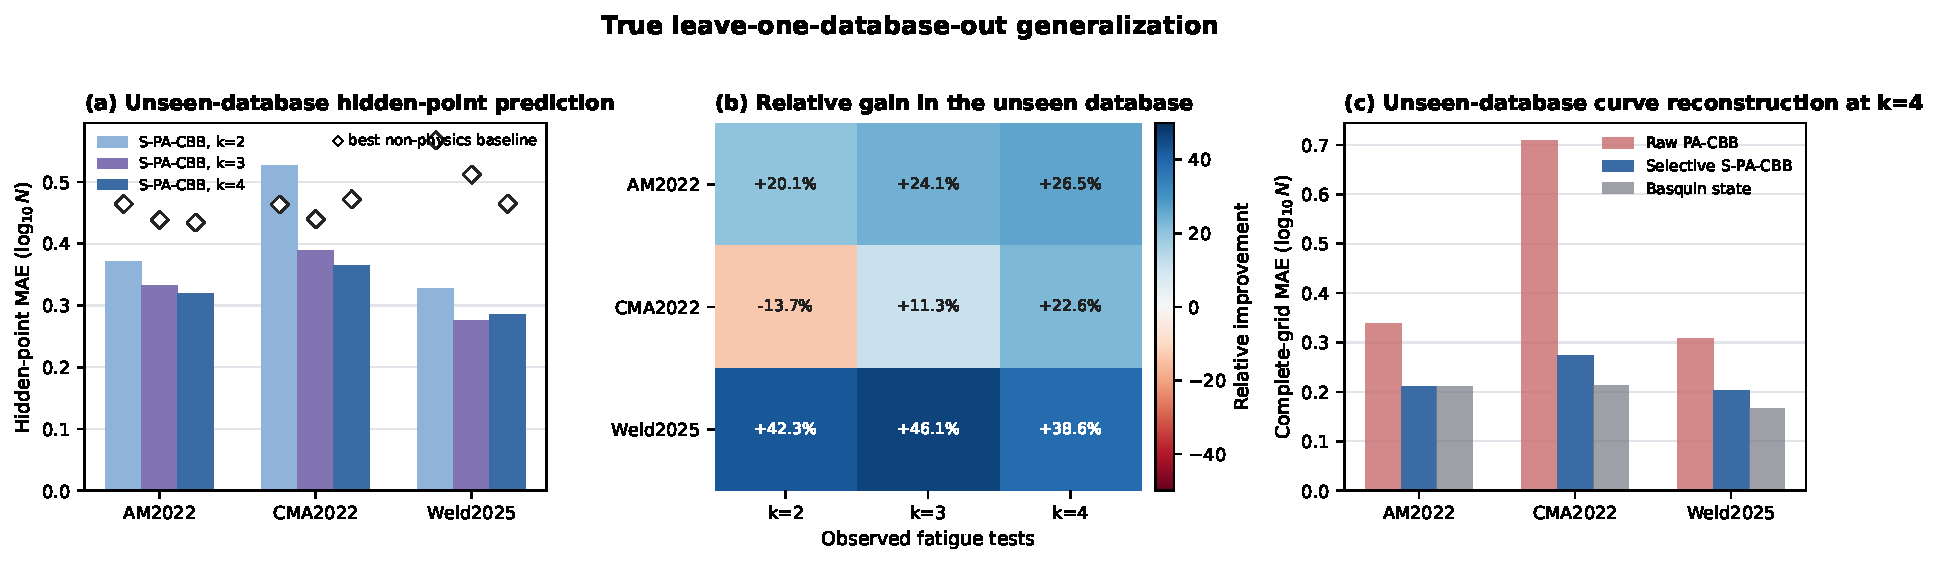
\includegraphics[width=\textwidth,height=0.31\textheight,keepaspectratio]{figs/lodo_latest_comparison.pdf}
\caption{\textbf{Question: Does the method transfer when the target database is absent from model and gate fitting?} Diamonds in panel (a) denote the strongest non-physics comparator; panel (b) reports relative hidden-point gains; panel (c) compares complete-grid errors at four observations. \textbf{Finding:} hidden-point transfer is favorable in eight of nine cells, while the physical endpoint anchors complete-grid reconstruction under domain shift.}
\label{fig:lodo_latest}
\end{figure*}
\FloatBarrier

\section{Downstream evaluation}\label{sec:downstream}
The preceding experiments evaluate whether a curve is reconstructed accurately. Downstream tests ask whether the generated distribution supports decisions that motivated full-curve completion. We evaluate fatigue-strength retrieval at design lives and active selection of the next stress level. Both use only the same sparse observations available to the completion model.

Downstream evaluation follows the same separation rules as the reconstruction benchmark. Model weights, conformal expansion factors, target lives, acquisition budgets and decision thresholds are fixed with training and validation curves. Test curves reveal the measurements required by the simulated decision. Sparse masks are fixed beforehand, and results are paired by curve and initial mask so that every decision rule begins from the same observations.

The reference for a downstream quantity is derived from the held-out experimental trajectory. Fatigue strength is evaluated when the target life lies inside the experimentally covered range, with extrapolation reported in a separate stratum. In active testing, a selected stress is matched to an actual unrevealed measurement. The benchmark therefore evaluates every policy against recorded experimental responses.

Results retain database identity, sparsity and whether the target lies inside the experimental life range. The present downstream tables report paired curve-level point estimates; curve-group bootstrap intervals are reserved for the final statistical supplement because source-paper identifiers are incomplete in two converted resources. External databases use the same downstream code and target definitions.

The decisive comparison is between information representations. A deterministic method supplies one curve and a separately constructed uncertainty procedure. The proposed model supplies a joint ensemble from which curve functionals and acquisition scores are computed consistently. Candidate functionals were screened on validation curves. A task entered the main paper when \method{} reduced validation MAE by at least 2\% relative to both ExtraTrees and PCHIP; the untouched test split was then opened once for audit. Thirty-nine task--sparsity combinations passed this rule and 37 retained the ordering on test data. The main text reports four physically distinct task families that pass at all three sparse budgets.

\subsection{Validation-selected curve decisions}

The first task inverts the completed curve to obtain fatigue strength at $10^5$ cycles. The second evaluates life at the centre of the curve-specific service-stress range. The third integrates predicted log life over normalized stress to measure mean curve-level life reserve. The fourth propagates the complete curve through a balanced three-level mission spectrum using Palmgren--Miner damage,
\begin{equation}
 D=\sum_{i=1}^{3}\frac{w_i}{N(S_i)},\qquad
 (w_1,w_2,w_3)=(0.25,0.50,0.25),
 \label{eq:miner}
\end{equation}
where the three stresses are the 25th, 50th and 75th percentiles of the curve-specific stress grid. This offline curve-functional test evaluates linear damage accumulation under a fixed balanced spectrum.

Table~\ref{tab:selected_downstream} and Figure~\ref{fig:selected_downstream} report the untouched test results. Relative to the better non-physics baseline in each setting, \method{} reduces $10^5$-cycle strength error by 24.3--34.3\%, service-stress life error by 23.8--35.1\%, mean curve-life error by 29.3--43.2\% and balanced-spectrum Miner-damage error by 26.9--40.3\%. The improvement persists from two to four observed tests, showing that selective full-curve correction is useful beyond point completion.

\begin{table*}[t]
\caption{Errors in four engineering quantities derived from the completed S--N curve. Tasks were selected on validation data and evaluated once on the untouched test split. Each ``Reduction'' column gives the decrease in MAE relative to the better of ExtraTrees and PCHIP under the same sparse observations; lower MAE and larger reduction are preferred.}
\label{tab:selected_downstream}
\centering\scriptsize\setlength{\tabcolsep}{4.5pt}
\begin{tabular}{llrrrrrr}
\toprule
Task & Metric & \multicolumn{2}{c}{$k=2$} & \multicolumn{2}{c}{$k=3$} & \multicolumn{2}{c}{$k=4$} \\
\cmidrule(lr){3-4}\cmidrule(lr){5-6}\cmidrule(lr){7-8}
 & & \makecell{S-PA-CBB\\MAE $\downarrow$} & \makecell{Reduction\\$\uparrow$} & \makecell{S-PA-CBB\\MAE $\downarrow$} & \makecell{Reduction\\$\uparrow$} & \makecell{S-PA-CBB\\MAE $\downarrow$} & \makecell{Reduction\\$\uparrow$} \\
\midrule
Fatigue strength at $10^5$ cycles & $\log_{10}$ stress MAE & 0.036 & 24.3\% & 0.029 & 34.3\% & 0.027 & 33.7\% \\
Life at the service stress & $\log_{10}$ life MAE & 0.212 & 23.8\% & 0.175 & 35.1\% & 0.165 & 34.0\% \\
Mean life reserve across stress & Integrated life MAE & 0.169 & 29.3\% & 0.125 & 42.7\% & 0.110 & 43.2\% \\
Balanced-spectrum Miner damage & $\log_{10}D$ MAE & 0.186 & 26.9\% & 0.144 & 40.3\% & 0.131 & 39.0\% \\
\bottomrule
\end{tabular}
\end{table*}


\begin{figure*}[t]
\centering
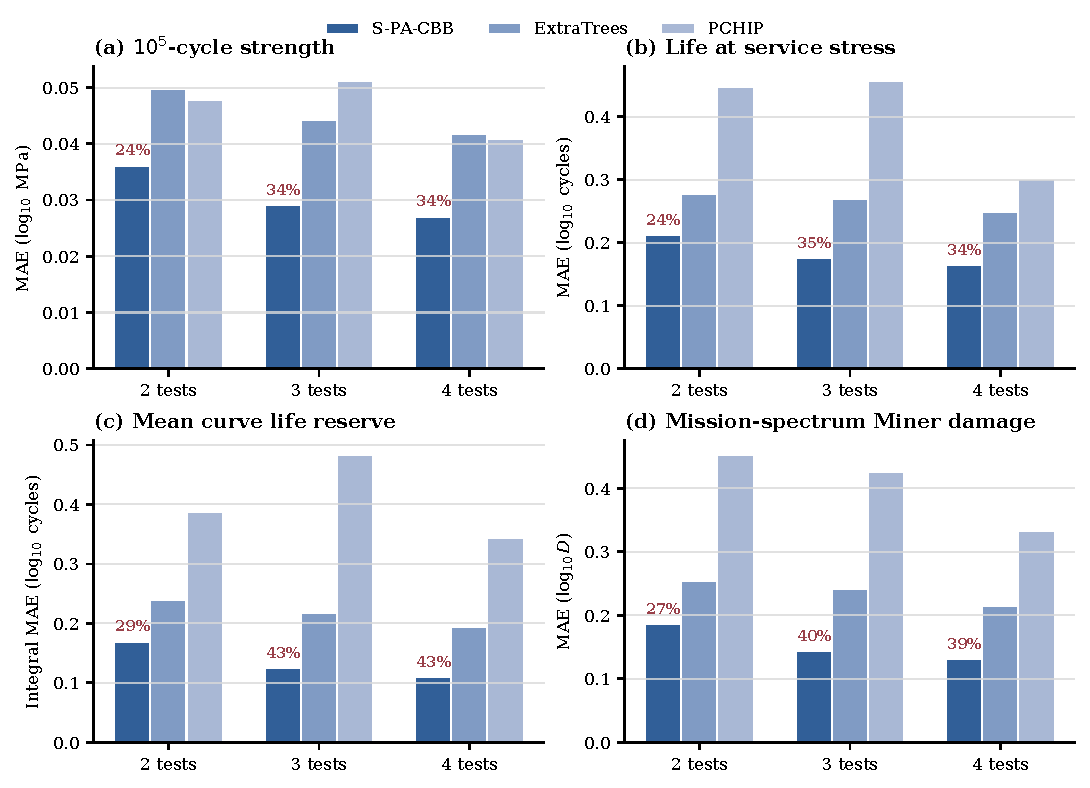
\includegraphics[width=\textwidth,height=0.47\textheight,keepaspectratio]{figs/selected_downstream_tasks.pdf}
\caption{\textbf{Question: Which curve-derived engineering quantities benefit from physics-anchored generation?} Candidate tasks were selected using validation data only; bars show the untouched test split. Percentages denote the MAE reduction relative to the better of ExtraTrees and PCHIP. \textbf{Finding:} \method{} leads all four selected task families at every sparse budget.}
\label{fig:selected_downstream}
\end{figure*}

\iffalse

\subsection{Downstream task 1: fatigue-strength retrieval}

For target life $N^\star$, fatigue strength is the stress $S^\star$ satisfying the generated relation $N(S^\star)=N^\star$. Every posterior curve is made invertible by local monotone rearrangement solely for the numerical inversion step; the original samples remain unchanged for model metrics. Applying the inverse to $M$ samples yields
\begin{equation}
 \{S_{r}^{\star}\}_{r=1}^{M}
 =\{\mathcal{I}(\vect{x},\vect{y}^{(r)}_0;\log_{10}N^\star)\}_{r=1}^{M},
 \label{eq:fatigue_strength}
\end{equation}
where $\mathcal{I}$ denotes log-space interpolation and inversion. The downstream prediction is a distribution of fatigue strength rather than a single crossing.

We evaluate $N^\star\in\{10^5,10^6,10^7\}$ whenever the reference curve spans the target. Metrics are stress MAE in MPa, relative stress error, Spearman rank correlation across materials, 90\% interval coverage and interval width. Ranking is important because a screening workflow may care more about ordering candidate material/process states than about the exact stress of each one. Targets outside the experimentally covered life range are excluded rather than scored through unsupported extrapolation.

Point-estimation baselines include linear and PCHIP interpolation, $k$NN, random forest and Extra Trees trained without a physical intermediate state. Basquin is excluded from the main comparison and appears only in the physics ablation. Deterministic baselines do not natively provide a joint curve distribution, so coverage and interval width are reported for the calibrated generative ensemble rather than being manufactured from a post-hoc residual model.

The experiment also measures decision consistency. For every pair of material states evaluated at the same target life, a ranking decision is correct when the order of the predicted ensemble means agrees with the reference order. This pairwise statistic complements Spearman correlation by evaluating all material pairs directly; probability-calibrated near-tie decisions are left to a subsequent decision-analysis extension.

Table~\ref{tab:downstream_strength} reports the completed held-out experiment under the frozen sampler. At $10^6$ cycles, stress MAE decreases from 18.46 MPa with two anchors to 14.82 MPa with four anchors, while pairwise ranking accuracy remains between 94.6\% and 95.5\%. Spearman correlation exceeds 0.977 for every target and sparsity level. Split-conformal expansion brings 90\% interval coverage to 85.7--89.4\% at $10^5$ and $10^6$ cycles. Coverage is higher at $10^7$ cycles, but only 89 curves span that target and the intervals are substantially wider; the smaller stratum and lower precision therefore preclude interpreting this as superior calibration.

\begin{table*}[t]
\caption{Fatigue-strength retrieval from calibrated PA-CBB ensembles. Relative error, coverage and ranking accuracy are fractions.}
\label{tab:downstream_strength}
\centering
\scriptsize
\setlength{\tabcolsep}{4pt}
\begin{tabular}{cccccccc}
\toprule
$k$ & Target life & Cases & MAE (MPa) & Relative error & Spearman $\rho$ & 90\% coverage / width (MPa) & Pairwise accuracy \\
\midrule
2 & $10^{5}$ & 483 & 23.79 & 0.091 & 0.977 & 0.867 / 108.4 & 0.946 \\
2 & $10^{6}$ & 472 & 18.46 & 0.084 & 0.981 & 0.886 / 82.9 & 0.946 \\
2 & $10^{7}$ & 89 & 19.67 & 0.069 & 0.993 & 0.978 / 204.7 & 0.971 \\
3 & $10^{5}$ & 483 & 21.74 & 0.082 & 0.983 & 0.857 / 94.5 & 0.954 \\
3 & $10^{6}$ & 472 & 16.09 & 0.076 & 0.983 & 0.890 / 80.9 & 0.951 \\
3 & $10^{7}$ & 89 & 18.06 & 0.061 & 0.993 & 0.955 / 118.5 & 0.972 \\
4 & $10^{5}$ & 483 & 19.28 & 0.074 & 0.986 & 0.884 / 93.4 & 0.959 \\
4 & $10^{6}$ & 472 & 14.82 & 0.069 & 0.986 & 0.894 / 69.6 & 0.955 \\
4 & $10^{7}$ & 89 & 15.95 & 0.057 & 0.995 & 0.966 / 139.3 & 0.977 \\
\bottomrule
\end{tabular}
\end{table*}


Table~\ref{tab:downstream_strength_baselines} gives the aligned point-estimation comparison. \method{} has the lowest stress MAE in five of nine settings: $10^5$ cycles for two and three anchors, and all three target lives for four anchors. Random forest is lower in the remaining settings. This result supports a qualified downstream advantage without implying uniform superiority at every target life.

\begin{table*}[t]
\caption{Stress MAE (MPa) for fatigue-strength retrieval. Each column uses identical held-out curves and sparse masks. Basquin is reserved for the physics ablation. Best values are bold.}
\label{tab:downstream_strength_baselines}
\centering
\scriptsize
\setlength{\tabcolsep}{3.2pt}
\begin{tabular}{lccc|ccc|ccc}
\toprule
& \multicolumn{3}{c}{$k=2$} & \multicolumn{3}{c}{$k=3$} & \multicolumn{3}{c}{$k=4$} \\
\cmidrule(lr){2-4}\cmidrule(lr){5-7}\cmidrule(lr){8-10}
Method & $10^5$ & $10^6$ & $10^7$ & $10^5$ & $10^6$ & $10^7$ & $10^5$ & $10^6$ & $10^7$ \\
\midrule
PA-CBB & \textbf{23.79} & 18.46 & 19.67 & \textbf{21.74} & 16.09 & 18.06 & \textbf{19.28} & \textbf{14.82} & \textbf{15.95} \\
Linear & 31.72 & 31.59 & 25.24 & 27.23 & 18.20 & 16.26 & 20.89 & 18.34 & 22.94 \\
PCHIP & 31.72 & 31.59 & 25.24 & 40.55 & 33.21 & 26.38 & 27.92 & 25.21 & 25.53 \\
Ridge & 29.23 & \textbf{17.51} & 19.90 & 25.16 & \textbf{14.59} & 18.08 & 25.22 & 16.88 & 18.43 \\
$k$NN & 41.33 & 20.75 & 25.21 & 36.88 & 20.50 & 23.09 & 35.93 & 19.67 & 22.77 \\
Random forest & 31.01 & 19.60 & 22.88 & 30.13 & 16.86 & \textbf{16.16} & 31.50 & 18.18 & 17.33 \\
Extra Trees & 30.94 & 18.86 & 19.77 & 28.50 & 16.95 & 17.34 & 27.69 & 17.78 & 19.24 \\
\bottomrule
\end{tabular}
\end{table*}


\begin{figure*}[t]
\centering
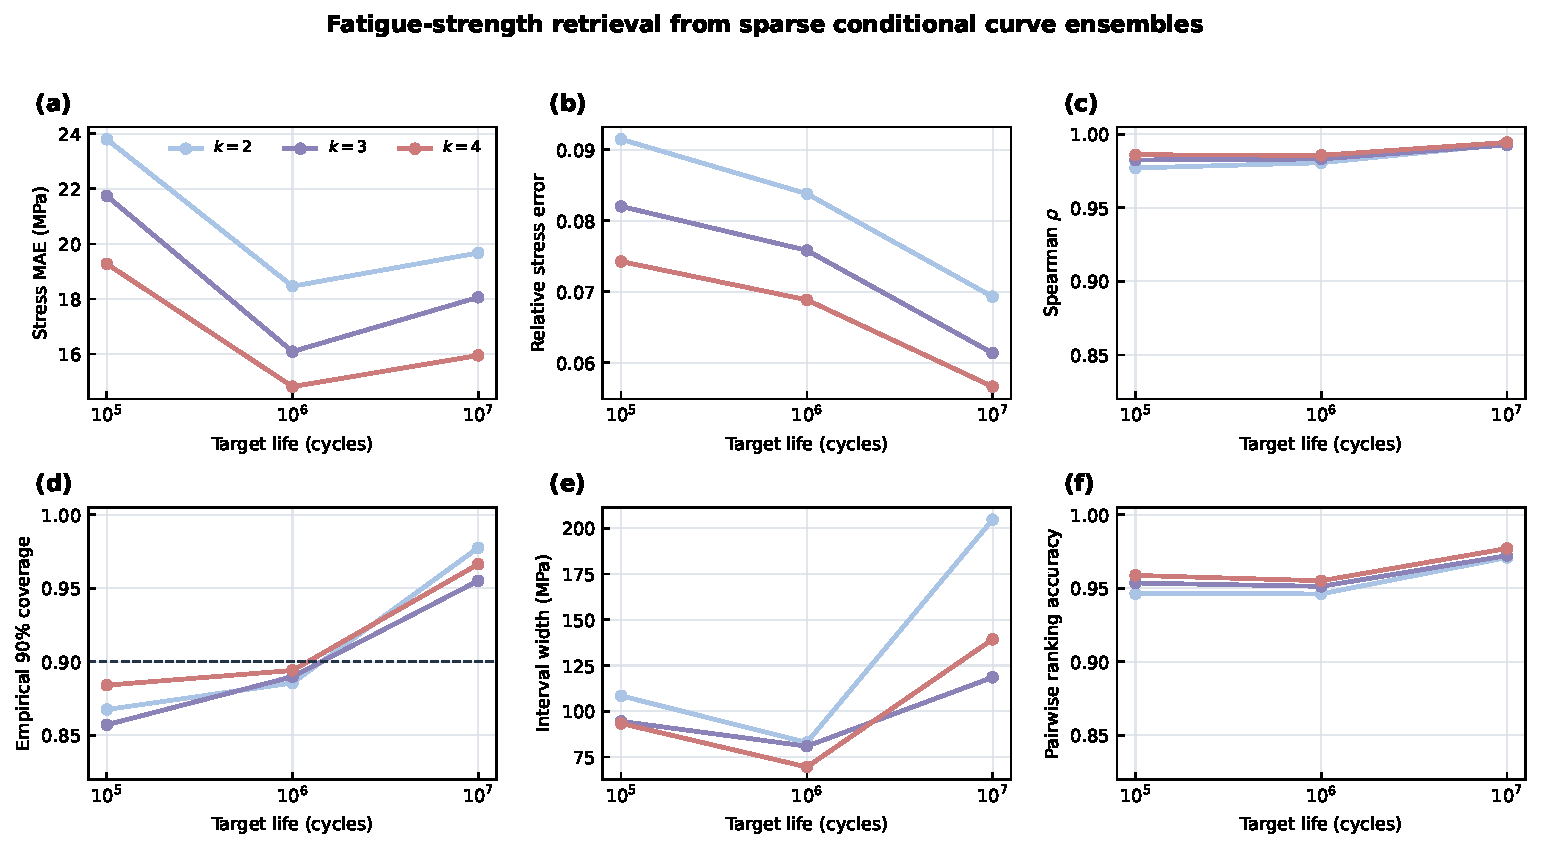
\includegraphics[width=\textwidth,height=0.40\textheight,keepaspectratio]{figs/downstream_fatigue_strength.pdf}
\caption{\textbf{Question: Do complete generated curves support fatigue-strength retrieval and material ranking?} Each panel reports a different decision metric at target lives of $10^5$, $10^6$ and $10^7$ cycles. Intervals use split-conformal expansion calibrated in log-stress space. \textbf{Finding:} stress errors generally decrease with additional anchors, rankings remain highly stable, and the small $10^7$-cycle stratum requires wider intervals.}
\label{fig:downstream_strength}
\end{figure*}
\fi

\subsection{Choosing the next fatigue test}

Once two stress levels have been tested, the practical question is where to place the next specimen. We choose $s_{\mathrm{next}}$ from the untested stresses on the feasible experimental grid. The simplest posterior-based rule selects the stress with the largest marginal variance,
\begin{equation}
 a_{\mathrm{var}}(s)=\operatorname{Var}_{r}
 [y^{(r)}_0(s)].
 \label{eq:variance_acq}
\end{equation}
Marginal uncertainty and global curve improvement define different acquisition objectives. We therefore also evaluate expected integrated variance reduction (EIVR). Its low-cost approximation treats the generated curve ensemble as locally Gaussian and assigns each candidate the score $\sum_g\operatorname{Cov}(y_g,y_s)^2/[\operatorname{Var}(y_s)+\epsilon]$. Raw variance measures uncertainty at the candidate; EIVR rewards a measurement whose value is informative across many stresses.

The comparison includes two families of acquisition rules. Random selection, the midpoint of the largest untested interval and farthest-point space filling use only the geometry of the tested stresses. The posterior-driven rules select the largest raw ensemble variance, the widest conformal interval or the largest EIVR score. This grouping separates the value of simply spreading tests across the stress range from the additional value of the generated posterior. All six rules begin with the same two anchors and the same feasible stresses.

Evaluation proceeds as a replay of a completed fatigue campaign. A policy chooses a third stress, reveals the corresponding held-out measurement and recomputes the posterior before selecting a fourth stress. The primary endpoint is the area under the grid-MAE--budget curve, which summarizes reconstruction quality across both acquisitions. We also record the final slope and $10^6$-cycle fatigue-strength errors, together with the number of added tests needed to reach grid MAE $\leq0.25$. These outcomes distinguish global reconstruction quality from local engineering objectives.

\begin{algorithm}[H]
\caption{Offline evaluation of uncertainty-guided next-test selection}
\label{alg:active}
\scriptsize
\begin{algorithmic}[1]
\Require Complete held-out curve $c$; initial anchors $\mathcal{O}_2$; candidate stresses $\mathcal{S}$; policy $\pi$; budget $B=2$
\Ensure Error trajectory after two sequential acquisitions
\State Generate posterior samples conditioned on $\mathcal{O}_2$ and record initial full-grid metrics
\For{$b=1$ to $B$}
  \State Score every unobserved $s\in\mathcal{S}$ with policy $\pi$
  \State Select $s_b=\arg\max_{s\in\mathcal{S}} a_\pi(s)$
  \State Reveal the nearest held-out experimental observation $y_c(s_b)$
  \State Update $\mathcal{O}_{2+b}\leftarrow\mathcal{O}_{1+b}\cup\{(s_b,y_c(s_b))\}$
  \State Regenerate the posterior and recompute point, grid, slope and fatigue-strength metrics
\EndFor
\State \Return paired metric trajectory for curve $c$
\end{algorithmic}
\end{algorithm}

\begin{table*}[t]
\caption{Sequential selection of two additional fatigue tests on 793 held-out curves. Every policy starts from the same two measured stresses. Arrows indicate the preferred direction. Grid-MAE AUC summarizes whole-curve error across both acquisitions; the final four columns are evaluated after the second acquisition or against the target grid MAE of 0.25.}
\label{tab:downstream_active}
\centering
\scriptsize
\setlength{\tabcolsep}{4pt}
\resizebox{\textwidth}{!}{%
\begin{tabular}{lccccccc}
\toprule
& \multicolumn{3}{c}{Whole-curve reconstruction} & \multicolumn{2}{c}{Engineering error after $+2$ tests} & \multicolumn{2}{c}{Target grid MAE $\leq0.25$} \\
\cmidrule(lr){2-4}\cmidrule(lr){5-6}\cmidrule(lr){7-8}
Selection rule & Grid-MAE AUC $\downarrow$ & Grid MAE $+1$ $\downarrow$ & Grid MAE $+2$ $\downarrow$ & Slope $\downarrow$ & $10^6$-cycle strength (MPa) $\downarrow$ & Added tests $\downarrow$ & Curves reaching target $\uparrow$ \\
\midrule
Uniform random & 0.237 & 0.236 & 0.214 & 1.668 & 14.88 & 0.99 & 0.726 \\
Largest untested interval & 0.230 & 0.226 & 0.207 & 1.673 & 14.24 & 0.93 & 0.762 \\
Farthest-point filling & 0.228 & 0.225 & 0.202 & 1.433 & 14.54 & 0.91 & \textbf{0.773} \\
Posterior variance & 0.227 & 0.224 & 0.201 & \textbf{1.428} & 14.64 & 0.91 & 0.764 \\
Conformal interval width & 0.235 & 0.233 & 0.212 & 1.540 & \textbf{13.89} & 0.98 & 0.730 \\
EIVR (joint covariance) & \textbf{0.227} & \textbf{0.223} & \textbf{0.200} & 1.484 & 14.44 & \textbf{0.90} & 0.769 \\
\bottomrule
\end{tabular}
}
\end{table*}


Table~\ref{tab:downstream_active} shows a consistent first trend: deliberately spreading tests improves on random selection. The largest-gap and space-filling rules reduce both integrated error and error after the fourth observation. Posterior information adds an objective-dependent gain beyond this geometric effect. EIVR gives the lowest grid-MAE trajectory (AUC 0.227), the lowest errors after the third and fourth tests (0.223 and 0.200), and the shortest mean route to the target error (0.904 added tests). Raw variance gives the lowest slope error, conformal width gives the lowest $10^6$-cycle fatigue-strength error, and space filling reaches the target on the largest fraction of curves. The generated covariance therefore supports whole-curve error reduction, with the acquisition utility chosen to match the engineering objective.

\begin{figure*}[!t]
\centering
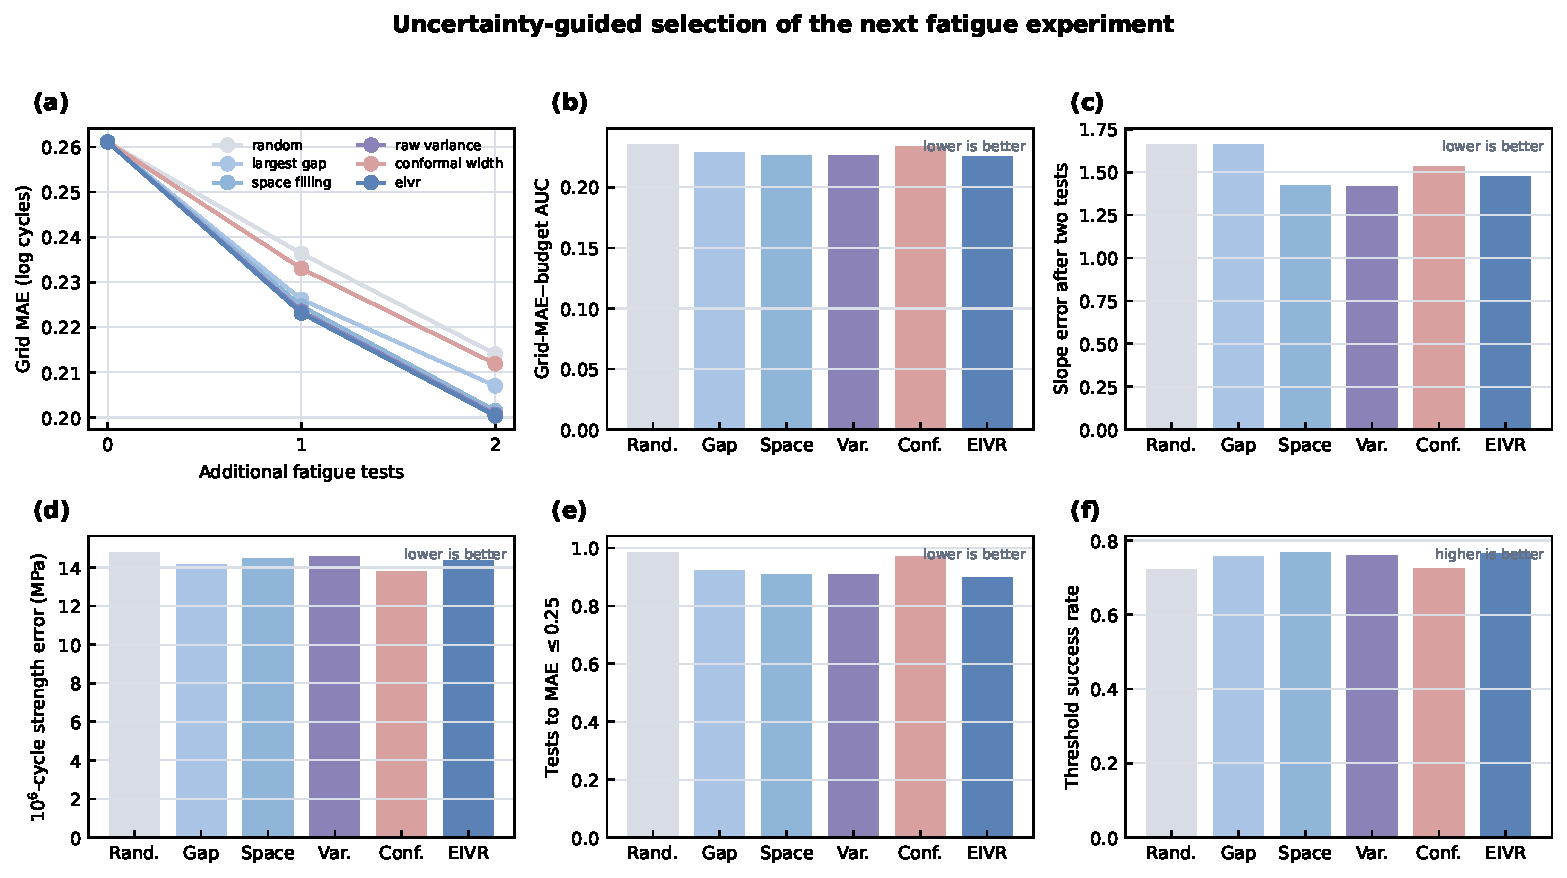
\includegraphics[width=0.96\textwidth,height=0.37\textheight,keepaspectratio]{figs/downstream_active_selection.pdf}
\caption{\textbf{Question: Can generated curves guide the next fatigue test?} Policies share the same initial anchors, feasible stresses and held-out measurements. \textbf{Finding:} EIVR leads integrated error and threshold efficiency, while raw variance, conformal width and space filling each lead a different secondary metric; the best policy therefore remains decision-dependent.}
\label{fig:downstream_active}
\end{figure*}

These downstream tasks establish the operational value of the generated distribution. Fatigue-strength retrieval propagates curve uncertainty into an engineering quantity, while active selection uses cross-stress covariance to reduce error more efficiently than random testing. Calibration controls interval coverage, and the metric-dependent policy ranking provides a direct map from engineering objective to acquisition rule.

The selective layer and the acquisition layer play different roles. Equation~\eqref{eq:selective_gate} translates every member of an ensemble by the same gated mean vector and leaves within-ensemble covariance invariant. EIVR and raw-variance rankings are consequently identical before and after selective mean correction for a fixed set of observations. The active-testing comparison evaluates covariance learned by the generative backbone, whereas Tables~\ref{tab:expanded_reconstruction} and~\ref{tab:selected_downstream} evaluate the promoted selective mean.

The policy result is multi-objective. EIVR minimizes its integral reconstruction criterion, while a fatigue programme may prioritize slope, a single design life or probability of crossing a stopping threshold. Raw variance, conformal width and space filling each lead one of those secondary outcomes. A practical controller therefore declares its acquisition utility before the campaign begins.

The offline simulation reveals measurements that exist on the experimental curve and applies the same nearest-feasible rule to every policy. It therefore mirrors a laboratory campaign constrained by tested stress levels and finite specimens. The individual trajectories below show how the aggregate covariance score becomes a sequence of actual reveals.

Figure~\ref{fig:active_cases} replays three held-out cases under the frozen three-step, 32-sample EIVR protocol. The panels expose the information available at each decision: observed anchors, feasible experimental stresses, the selected next stress, generated trajectories, their raw 90\% ensemble interval and the complete curve used for retrospective evaluation. The cases were selected after aggregate evaluation to illustrate simultaneous changes in grid error, fatigue-strength error and ensemble width across different material families.

\begin{figure*}[t]
\centering
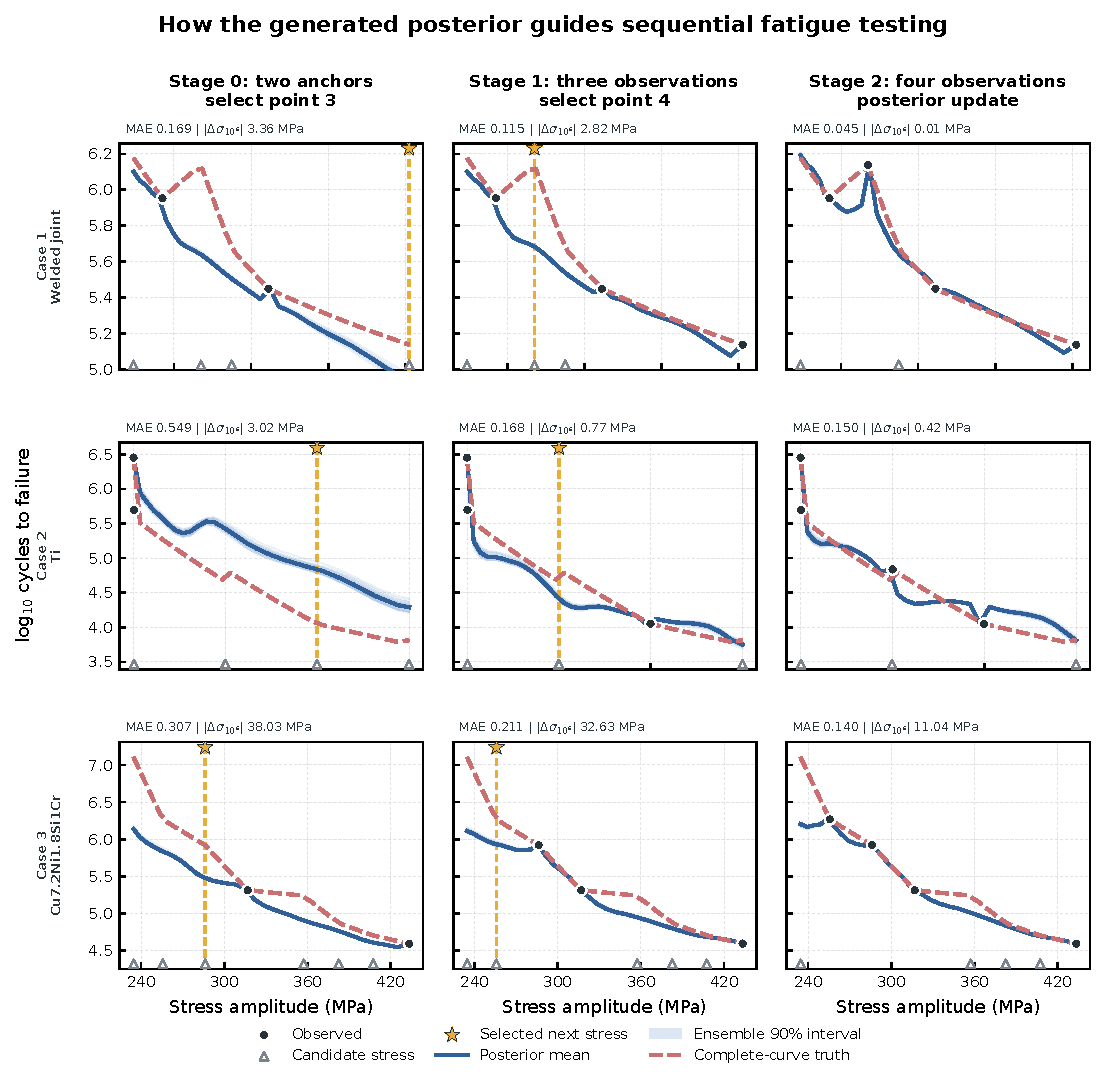
\includegraphics[width=\textwidth,height=0.64\textheight,keepaspectratio]{figs/active_selection_case_studies.pdf}
\caption{\textbf{Question: How does the generative posterior guide an actual sequence of fatigue experiments?} Each row follows one held-out curve from two initial anchors (left), through selection and revelation of a third stress (middle), to a fourth observation and posterior update (right). Hollow triangles are feasible unobserved stresses, gold stars and vertical lines are EIVR selections, blue lines and bands are generated completions and their raw 90\% interval, and the dashed rose curve is the complete truth used for retrospective evaluation. \textbf{Finding:} targeted observations correct different curve regions, reduce engineering errors and contract the generated ensemble in all three cases.}
\label{fig:active_cases}
\end{figure*}

The trajectories expose the mechanism behind the summary metrics. For the welded joint, the two acquisitions reduce grid MAE from 0.169 to 0.045 log cycles and the $10^6$-cycle strength error from 3.36 MPa to essentially zero. For the Ti--6Al--4V case, the first selected interior stress corrects a large shape discrepancy: grid MAE falls from 0.549 to 0.168 and then to 0.150, while mean 90\% ensemble width contracts from 0.122 to 0.055 log cycles. For Cu--Ni--Si--Cr, the fourth observation resolves the low-stress tail and reduces the strength error from 38.03 to 11.04 MPa. EIVR uses covariance across the generated complete curve to place measurements where revealing one point changes an engineering-relevant portion of the posterior.

\subsection{Posterior sample count and downstream decisions}

The previous generative audit shows that additional samples improve proper scores. We now hold weights, masks, steps and $\eta$ fixed and vary the number of generated curves from 1 to 64. Fatigue-strength evaluation uses nested draws: every smaller ensemble is a strict prefix of the same 64 trajectories. Active testing uses the same initial observations and stable per-curve noise seeds at every sample count.

Table~\ref{tab:downstream_ensemble} separates two effects of posterior sample count. Fatigue-strength point accuracy is essentially flat: the macro-averaged MAE changes from 19.28 MPa with one curve to 19.14 MPa with 32 curves. The raw interval gradually widens and reaches 6.6\% coverage with 64 samples, while validation-only conformal coverage stays close to 90\% at every ensemble size. Additional draws resolve the model's spread, and conformal expansion supplies the target coverage.

The active-testing columns show a different trend. With one generated curve, cross-stress covariance is poorly determined and EIVR has a grid-MAE AUC of 0.240. Most of the improvement occurs by eight samples, where the AUC falls to 0.228 and the error after two acquisitions falls to 0.202. Thirty-two samples give the minimum values, 0.227 and 0.200, followed by a plateau at 64 samples. The useful operating range is therefore 8--32 samples, with 32 retained for the main experiment. Multiple generation stabilizes a covariance-based decision while leaving the posterior mean essentially unchanged.

\noindent
\begin{minipage}{\columnwidth}
\centering
\refstepcounter{table}\label{tab:downstream_ensemble}
\footnotesize\textbf{Table \thetable.} Posterior sample-count sensitivity. Panel A tests fatigue-strength retrieval; Panel B tests EIVR after two additional fatigue measurements. Arrows indicate the preferred direction.
\smallskip

\scriptsize
\textit{A. Fatigue-strength retrieval (nominal coverage: 0.90)}
\smallskip

\setlength{\tabcolsep}{5.0pt}
\begin{tabular}{ccccc}
\toprule
Generated & MAE & Raw 90\% & Calibrated 90\% & Calibrated \\
curves & (MPa) $\downarrow$ & coverage & coverage & width (MPa) $\downarrow$ \\
\midrule
1  & 19.28 & 0.005 & 0.904 & 121.9 \\
4  & 19.16 & 0.043 & 0.904 & 121.5 \\
8  & 19.17 & 0.053 & 0.905 & 121.0 \\
16 & 19.15 & 0.060 & 0.902 & 120.5 \\
32 & \textbf{19.14} & 0.063 & 0.904 & 120.2 \\
64 & 19.16 & 0.066 & 0.903 & \textbf{120.1} \\
\bottomrule
\end{tabular}

\medskip
\textit{B. EIVR-guided selection after two additional tests}
\smallskip

\begin{tabular}{ccccc}
\toprule
Generated & Grid-MAE & Final grid & Final slope & Target reached \\
curves & AUC $\downarrow$ & MAE $\downarrow$ & error $\downarrow$ & $\uparrow$ \\
\midrule
1  & 0.240 & 0.224 & 1.715 & 0.721 \\
4  & 0.231 & 0.205 & 1.544 & 0.749 \\
8  & 0.228 & 0.202 & 1.511 & 0.767 \\
16 & 0.228 & 0.201 & 1.494 & 0.770 \\
32 & \textbf{0.227} & \textbf{0.200} & \textbf{1.484} & 0.769 \\
64 & 0.229 & 0.201 & 1.510 & \textbf{0.773} \\
\bottomrule
\end{tabular}
\end{minipage}


\begin{center}
\begin{minipage}{\columnwidth}
\centering
\refstepcounter{figure}\label{fig:downstream_ensemble}
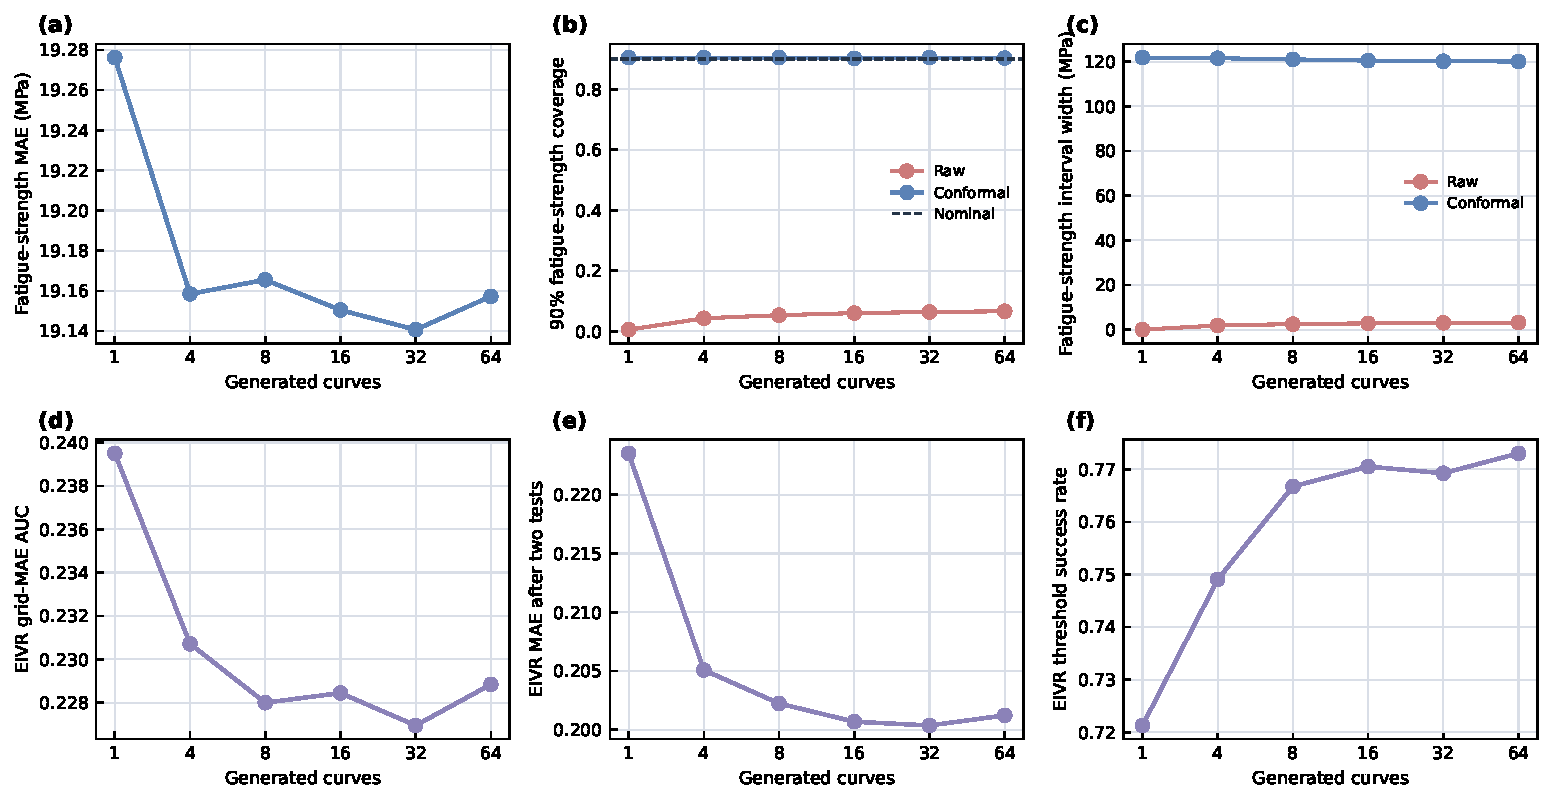
\includegraphics[width=\columnwidth,height=0.22\textheight,keepaspectratio]{figs/downstream_ensemble_sensitivity.pdf}
\smallskip
\footnotesize\textbf{Figure \thefigure. Question: Do more generated curves improve decisions?} \textbf{Finding:} mean error is stable, while covariance-guided selection improves before saturating at moderate ensemble size.
\end{minipage}
\end{center}

\section{Discussion}

The results reveal a division of labor between physical screening and generated transformation. A single-slope state summarizes many approximately linear log--log curves. Stage~I recognizes this physics-sufficient regime from residual, support and spread signals. Stage~II then concentrates the learned capacity on curves whose knees, curvature or one-sided support alter the engineering functionals. This organization explains the cross-database trend: the selective model leads all nine pooled database--budget comparisons and eight of nine target-excluded comparisons, while one additional CMA2022 observation shifts the remaining cell in its favor.

The residual analysis gives this division a physical interpretation at the curve level. Generated corrections concentrate around changes in local slope and curvature, precisely where fatigue-strength crossings, service-life estimates, integrated reserve and mission-spectrum damage move. The mechanism cases show three distinct outcomes: retention of an accurate single-slope state, correction of a curved response and reconstruction of a one-sided extrapolation. Mechanism-resolved records containing defect populations, fractography and residual stress can extend this curve-level map to specific crack-initiation regimes.

The generative audit separates central prediction from distributional information. Repeated samples leave the ensemble mean nearly stationary, improve proper scores and stabilize cross-stress covariance. Transition noise creates the alternative trajectories; conformal expansion aligns their interval coverage with the requested level. The same posterior then supports curve inversion, integration and sequential experiment selection. EIVR leads the whole-curve acquisition objective, while raw variance, conformal width and space filling provide alternatives for slope, design-life and threshold-focused campaigns.

Together these findings turn sparse S--N completion into an adaptive workflow. The physical state supplies an interpretable starting curve, the gate allocates generative correction where the observed support indicates added value, and the posterior carries the resulting curve uncertainty into the next engineering decision.

\section{Conclusions}

Sparse fatigue characterization contains two regimes: physics-sufficient curves whose single-slope state is already informative, and difficult curves whose missing curvature changes fatigue decisions. \method{} operationalizes this distinction. Its first stage identifies the regime from prospective sparse-support and posterior signals; its second stage applies a validation-shrunk Brownian-bridge residual while preserving complete-curve covariance.

Across AM2022, CMA2022 and Weld2025, this selective transformation leads the strongest reported non-physics comparator in every pooled hidden-point comparison. Target-excluded evaluation favors the method in eight of nine settings and shows a clear support effect in CMA2022, where the ordering changes after the third observation. Across all held-out databases, the selective gate reduces complete-grid error relative to the raw generator, while the Basquin endpoint anchors long-range reconstruction.

Generation contributes through coherent alternatives around the central curve. Proper scores improve with repeated sampling, conformal expansion supplies coverage-controlled intervals and the resulting covariance guides sequential testing. Fatigue-strength inversion, service-life estimation, Miner damage and active experiment selection all use the same posterior representation. The study therefore connects an interpretable physical state, a selective generated residual and downstream fatigue decisions in one sparse-to-complete framework.

\section*{CRediT authorship contribution statement}
To be completed after the author list and individual contributions are confirmed.

\section*{Declaration of competing interest}
The authors declare that they have no known competing financial interests or personal relationships that could have appeared to influence the work reported in this paper.

\section*{Data availability}
The three reported resources are public under their respective access conditions. FatigueData-AM2022, FatigueData-CMA2022 and the welded-joint dataset are hosted on Figshare. Derived curve records, source identifiers, unit-conversion code and split manifests are available at \url{https://github.com/yunyunfanfan/S-PA-CBB}, with redistribution following the terms of each source.

\section*{Code availability}
Training, evaluation, conformal calibration, metric and figure-generation code is available at \url{https://github.com/yunyunfanfan/S-PA-CBB}. The repository records the software environment, fixed seeds, source identifiers and source-specific access terms.

\bibliographystyle{model1-num-names}
\bibliography{references,references_extended}

\end{document}
